% Font options: 10pm, 11pt, 12pt
% Align headings left instead of center: nocenter
\documentclass[xcolor=x11names,compress]{beamer}\usepackage[]{graphicx}\usepackage[]{xcolor}
% maxwidth is the original width if it is less than linewidth
% otherwise use linewidth (to make sure the graphics do not exceed the margin)
\makeatletter
\def\maxwidth{ %
  \ifdim\Gin@nat@width>\linewidth
    \linewidth
  \else
    \Gin@nat@width
  \fi
}
\makeatother

\definecolor{fgcolor}{rgb}{0.345, 0.345, 0.345}
\newcommand{\hlnum}[1]{\textcolor[rgb]{0.686,0.059,0.569}{#1}}%
\newcommand{\hlstr}[1]{\textcolor[rgb]{0.192,0.494,0.8}{#1}}%
\newcommand{\hlcom}[1]{\textcolor[rgb]{0.678,0.584,0.686}{\textit{#1}}}%
\newcommand{\hlopt}[1]{\textcolor[rgb]{0,0,0}{#1}}%
\newcommand{\hlstd}[1]{\textcolor[rgb]{0.345,0.345,0.345}{#1}}%
\newcommand{\hlkwa}[1]{\textcolor[rgb]{0.161,0.373,0.58}{\textbf{#1}}}%
\newcommand{\hlkwb}[1]{\textcolor[rgb]{0.69,0.353,0.396}{#1}}%
\newcommand{\hlkwc}[1]{\textcolor[rgb]{0.333,0.667,0.333}{#1}}%
\newcommand{\hlkwd}[1]{\textcolor[rgb]{0.737,0.353,0.396}{\textbf{#1}}}%
\let\hlipl\hlkwb

\usepackage{framed}
\makeatletter
\newenvironment{kframe}{%
 \def\at@end@of@kframe{}%
 \ifinner\ifhmode%
  \def\at@end@of@kframe{\end{minipage}}%
  \begin{minipage}{\columnwidth}%
 \fi\fi%
 \def\FrameCommand##1{\hskip\@totalleftmargin \hskip-\fboxsep
 \colorbox{shadecolor}{##1}\hskip-\fboxsep
     % There is no \\@totalrightmargin, so:
     \hskip-\linewidth \hskip-\@totalleftmargin \hskip\columnwidth}%
 \MakeFramed {\advance\hsize-\width
   \@totalleftmargin\z@ \linewidth\hsize
   \@setminipage}}%
 {\par\unskip\endMakeFramed%
 \at@end@of@kframe}
\makeatother

\definecolor{shadecolor}{rgb}{.97, .97, .97}
\definecolor{messagecolor}{rgb}{0, 0, 0}
\definecolor{warningcolor}{rgb}{1, 0, 1}
\definecolor{errorcolor}{rgb}{1, 0, 0}
\newenvironment{knitrout}{}{} % an empty environment to be redefined in TeX

\usepackage{alltt}
%\documentclass[xcolor=x11names,compress,handout]{beamer}
\usepackage[]{graphicx}
\usepackage[]{color}
\usepackage{booktabs}
\usepackage{hyperref}
\usepackage{tikz}
\usepackage{multirow}
\usepackage{multicol}
\usepackage{dcolumn}
\usepackage{bigstrut}
\usepackage{amsmath} 
\usepackage{xcolor,colortbl}
\usepackage{amssymb}
%\newcommand{\done}{\cellcolor{teal}#1}

%% Beamer Layout %%%%%%%%%%%%%%%%%%%%%%%%%%%%%%%%%%
\useoutertheme[subsection=false,shadow]{miniframes}
\useinnertheme{default}
\usefonttheme{serif}
\usepackage{Arev}
\usepackage{pdfpages}

\setbeamerfont{title like}{shape=\scshape}
\setbeamerfont{frametitle}{shape=\scshape, size=\normalsize}

\definecolor{dkblue}{RGB}{0,0,102}

\setbeamercolor*{lower separation line head}{bg=dkblue} 
\setbeamercolor*{normal text}{fg=black,bg=white} 
\setbeamercolor*{alerted text}{fg=red} 
\setbeamercolor*{example text}{fg=black} 
\setbeamercolor*{structure}{fg=black} 
 
\setbeamercolor*{palette tertiary}{fg=black,bg=black!10} 
\setbeamercolor*{palette quaternary}{fg=black,bg=black!10} 

\renewcommand{\(}{\begin{columns}}
\renewcommand{\)}{\end{columns}}
\newcommand{\<}[1]{\begin{column}{#1}}
\renewcommand{\>}{\end{column}}

\setbeamertemplate{navigation symbols}{} 
\setbeamertemplate{footline}[frame number]
\setbeamertemplate{caption}{\raggedright\insertcaption\par}

\setbeamersize{text margin left=5pt,text margin right=5pt}

\setbeamercolor{block title}{use=structure,fg=white,bg=structure.fg!75!orange}
\setbeamercolor{block body}{parent=normal text,use=block title,bg=block title.bg!10!bg}

\AtBeginSection{\frame{\sectionpage}}
\usepackage{xcolor}
\hypersetup{
    colorlinks,
    linkcolor={red!50!black},
    citecolor={blue!50!black},
    urlcolor={blue!80!black}
}

%%%%%%%%%%%%%%%%%%%%%%%%%%%%%%%%%%%%%%%%%%%%%%%%%%




\title{Interpreting and Critiquing Causal Evidence}
\subtitle{Day 2 - Fundamental Critiques}
\author{Jonathan Phillips}
\IfFileExists{upquote.sty}{\usepackage{upquote}}{}
\begin{document}

\frame{\titlepage}

\section{Introduction}

\begin{frame}
\frametitle{What do political scientists \textbf{know}?}
\begin{itemize}
\item Door-to-door political campaigning works
\pause
\item Proportional Representation electoral systems have more parties
\pause
\item Democracies do not go to war with each other
\pause
\item Development helps democracies endure
\pause
\item ...And that's about it
\end{itemize}
\end{frame}

\begin{frame}
\frametitle{What do political scientists \textbf{know}?}
\begin{itemize}
\item Thousands of books and papers have \textit{not} generated much knowledge about what explains political outcomes
\pause
\begin{itemize}
\item Many add \textbf{descriptive} knowledge
\pause
\item Many investigate \textbf{specific} events, not generalizable variables
\pause
\item Many highlight \textbf{correlations} between variables
\end{itemize}
\end{itemize}
\end{frame}

\begin{frame}
\frametitle{Learning from Data}
\begin{itemize}
\item Why aren't case studies enough?
\pause
\begin{itemize}
\item If we want to know why some countries are more successful democracies than others, surely we have to examine the successful countries in detail?
\pause
\item Yes! But that's not \textit{sufficient}
\pause
\end{itemize}
\item The problem is that there are many variables that \textit{could} explain success
\pause
\item And detailed case studies can help us identify plausible \textit{hypotheses}
\pause
\item But the only way to \textit{confirm} the hypothesis is to verify that:
\pause
\begin{enumerate}
\item In other cases, the presence of the condition also produces the same outcome (if not, the explanation is not sufficient)
\pause
\item The absence of the condition does not produce the same outcome (if not, the explanation is not necessary)
\end{enumerate}
\end{itemize}
\end{frame}

\begin{frame}
\frametitle{Learning from Data}
\begin{itemize}
\item For example, we could look at India and conclude large Asian countries produce successful democracies
\pause
\begin{itemize}
\item But...China
\pause
\item But...Costa Rica
\pause
\end{itemize}
\item Only by looking at other cases, particularly 'control' cases (small non-Asian countries) can we understand if this explanation is plausible
\end{itemize}
\end{frame}

\begin{frame}
\frametitle{Learning from Data}
\begin{itemize}
\item Even when we compare multiple cases: 
\pause
\item \textbf{Correlation is not causation}
\pause
\begin{itemize}
\item If we look hard enough we can always find correlations
\pause
\item By chance...
\pause
\item Due to complex social patterns...
\pause
\item But we cannot conclude that there is a causal effect of $D$ on $Y$
\pause
\end{itemize}
\item \textit{More} data will not help
\pause
\item The problem is the \textit{type} of data; it does not allow us to answer the causal question 
\end{itemize}
\end{frame}

\setbeamercolor{background canvas}{bg=}
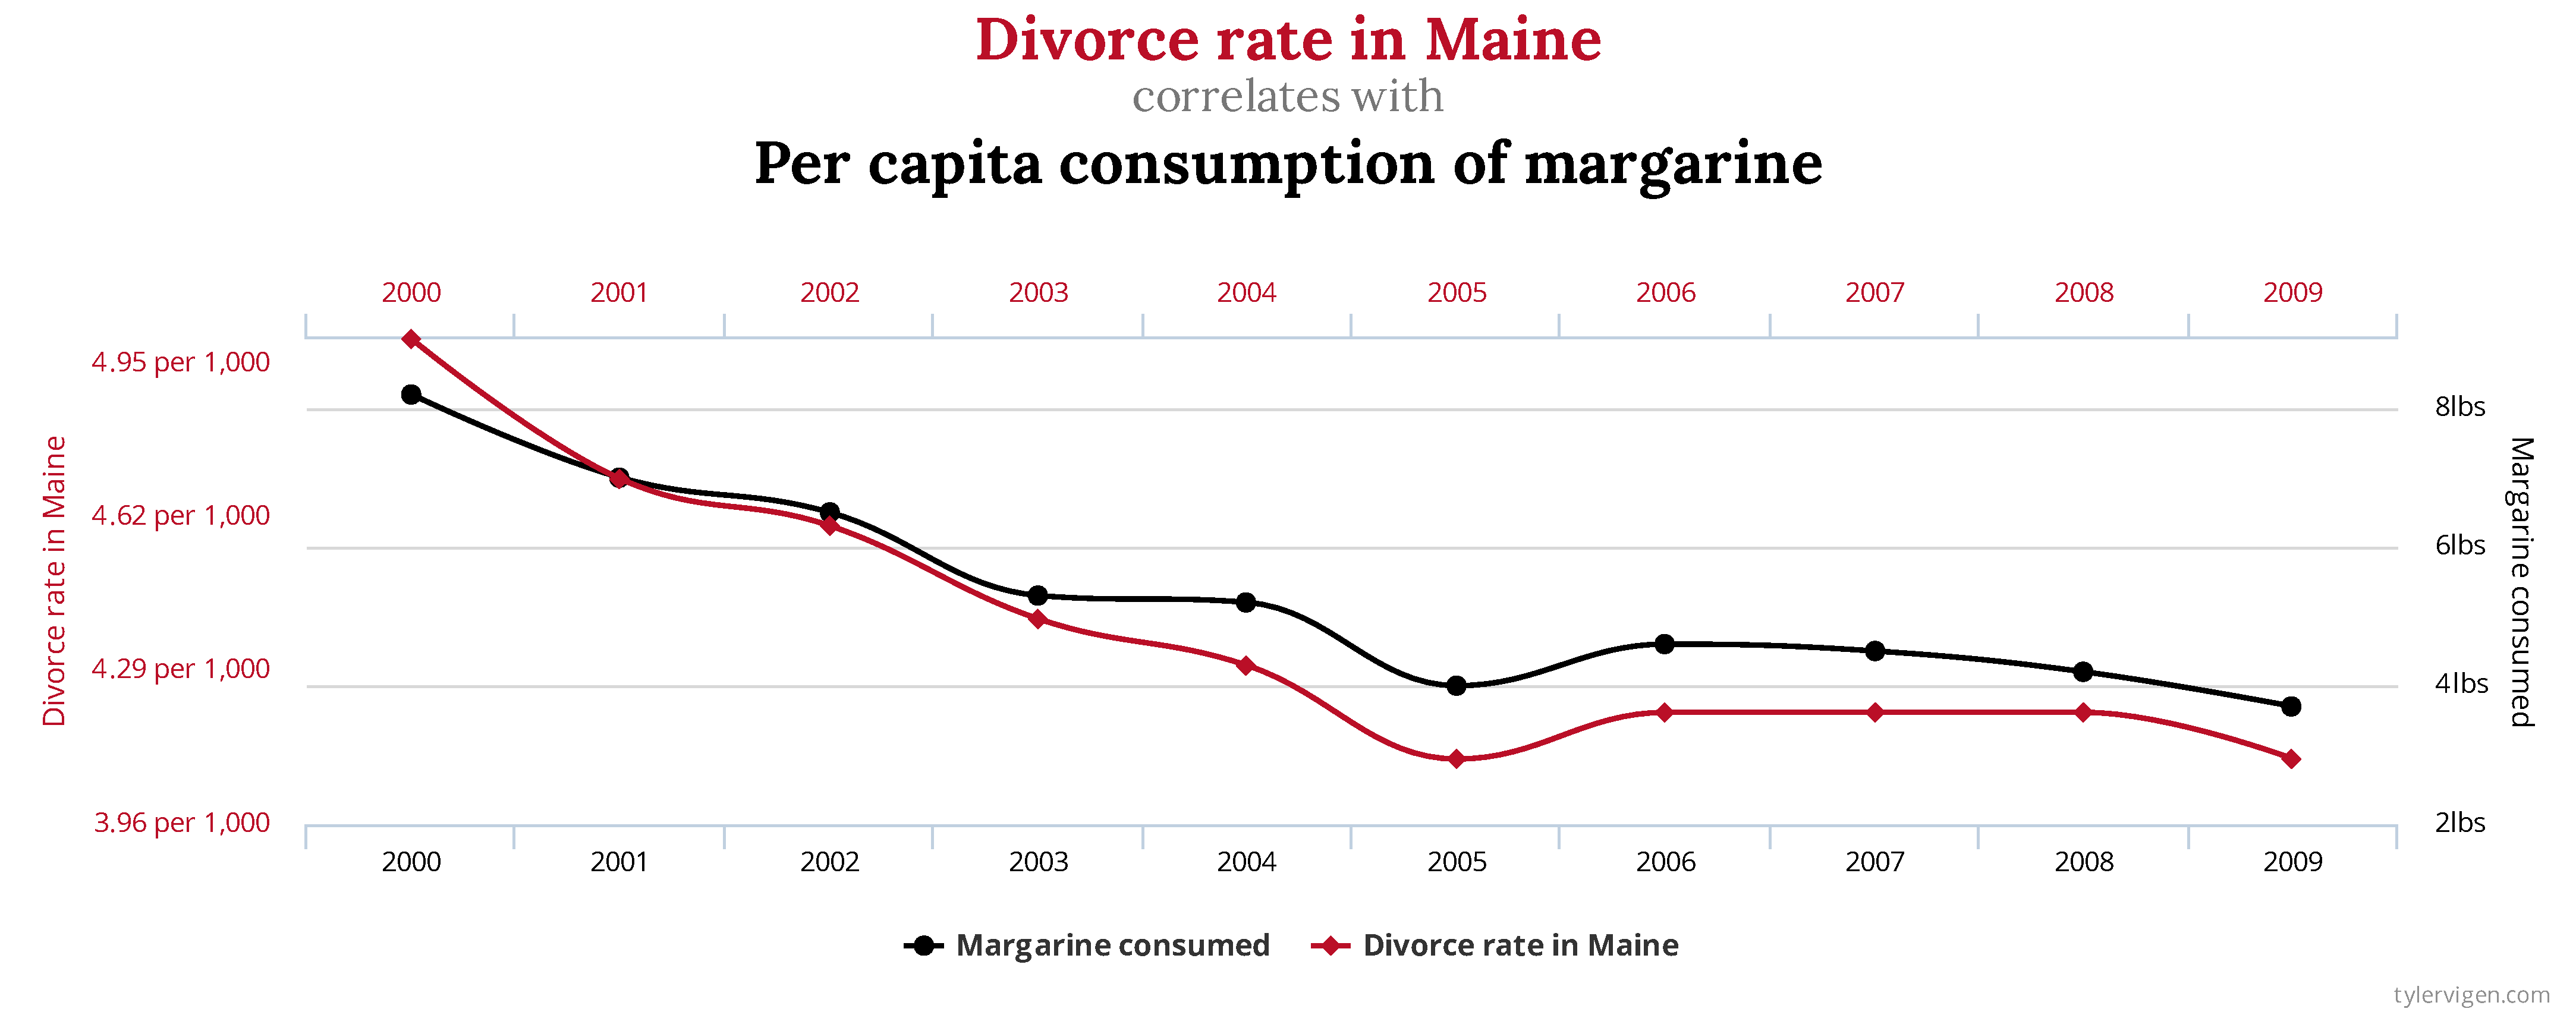
\includepdf[pages={1}]{chart_1.pdf}

\setbeamercolor{background canvas}{bg=}
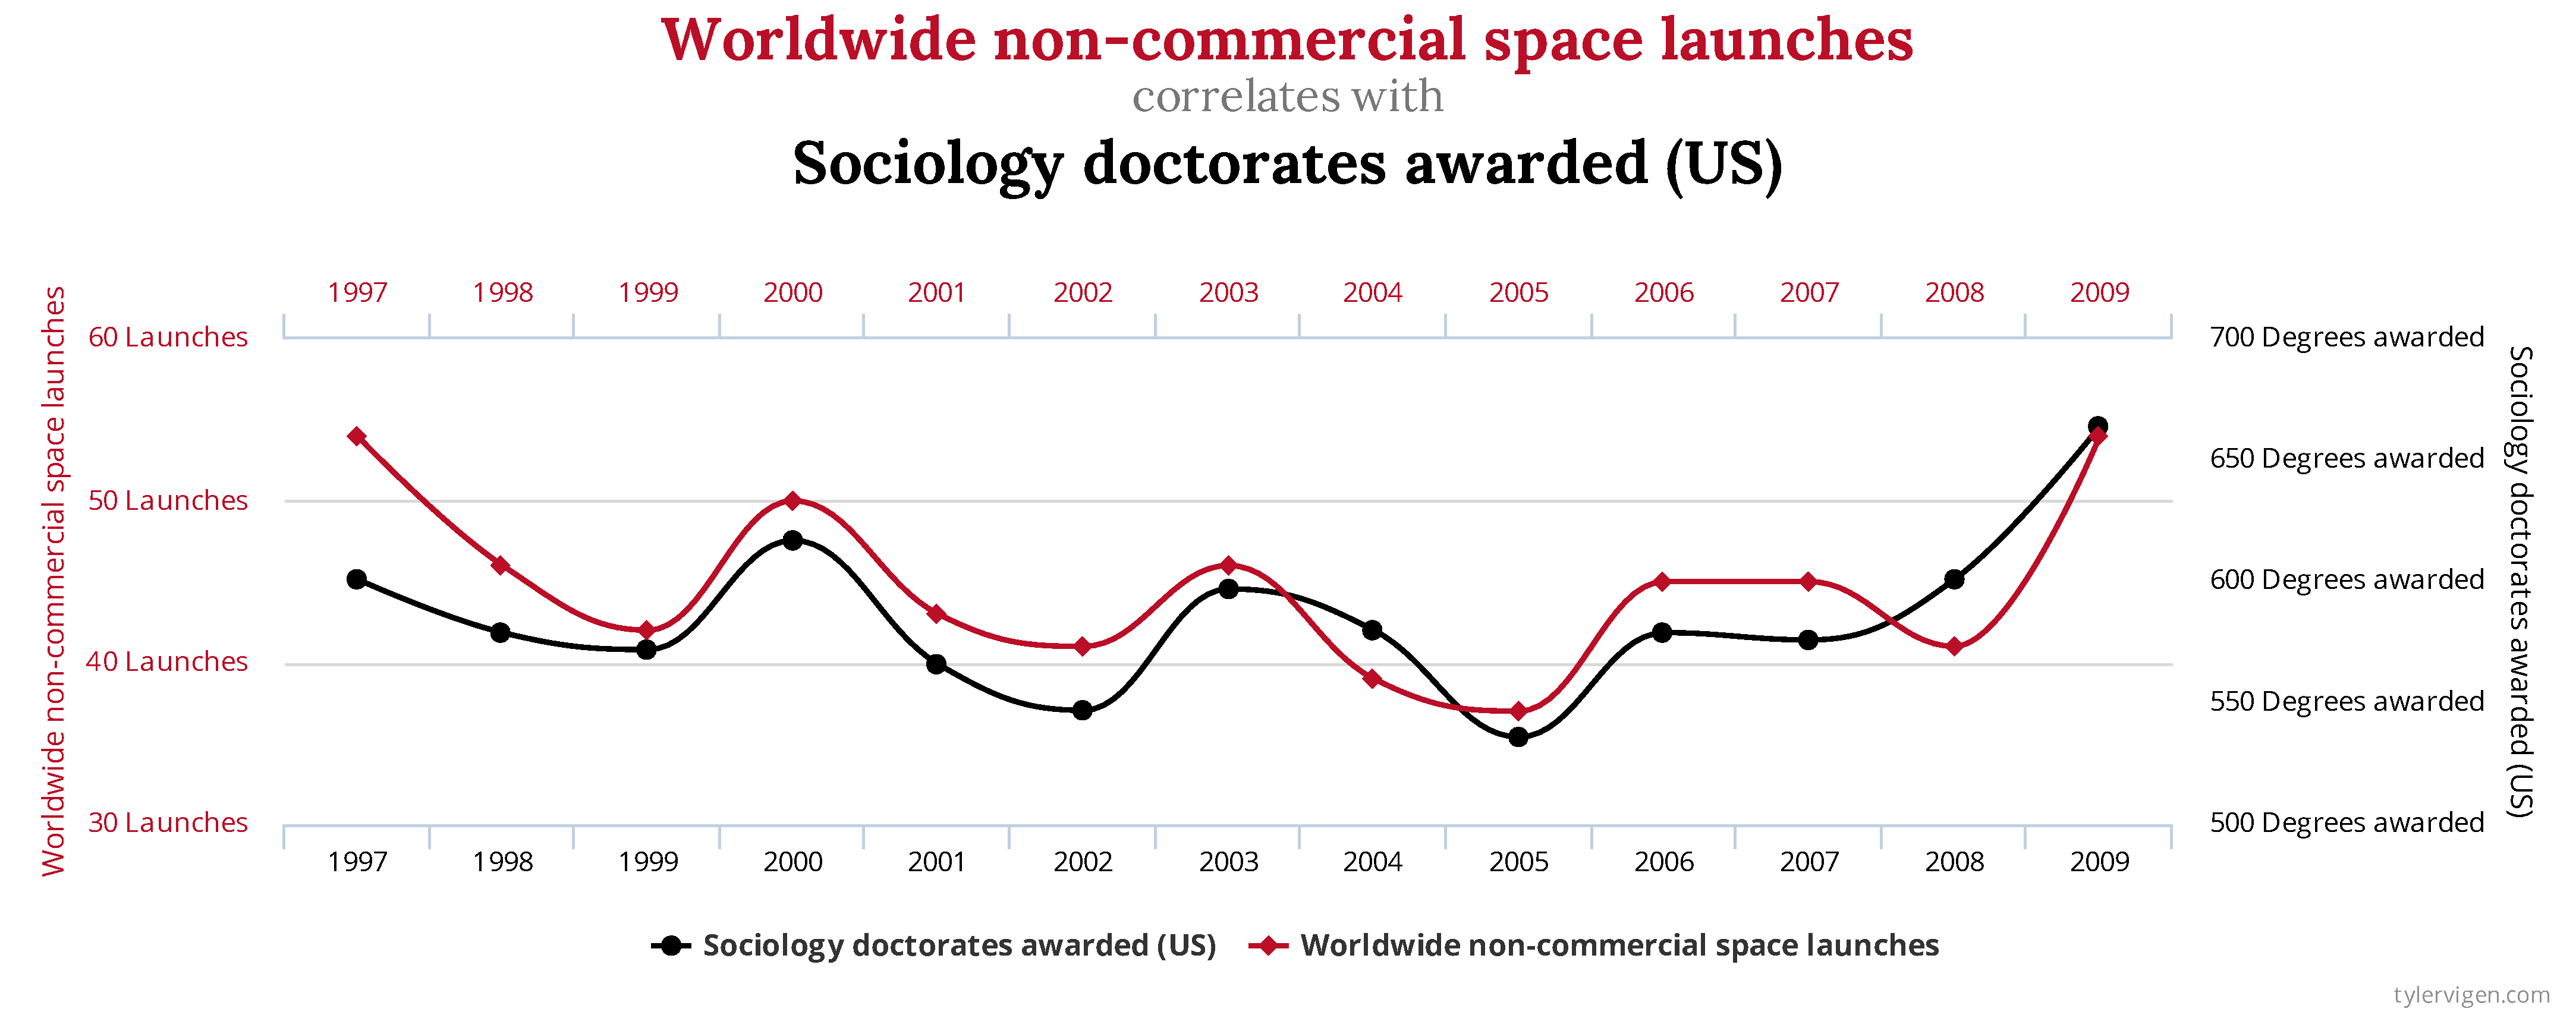
\includepdf[pages={1}]{chart_2.pdf}

\setbeamercolor{background canvas}{bg=}
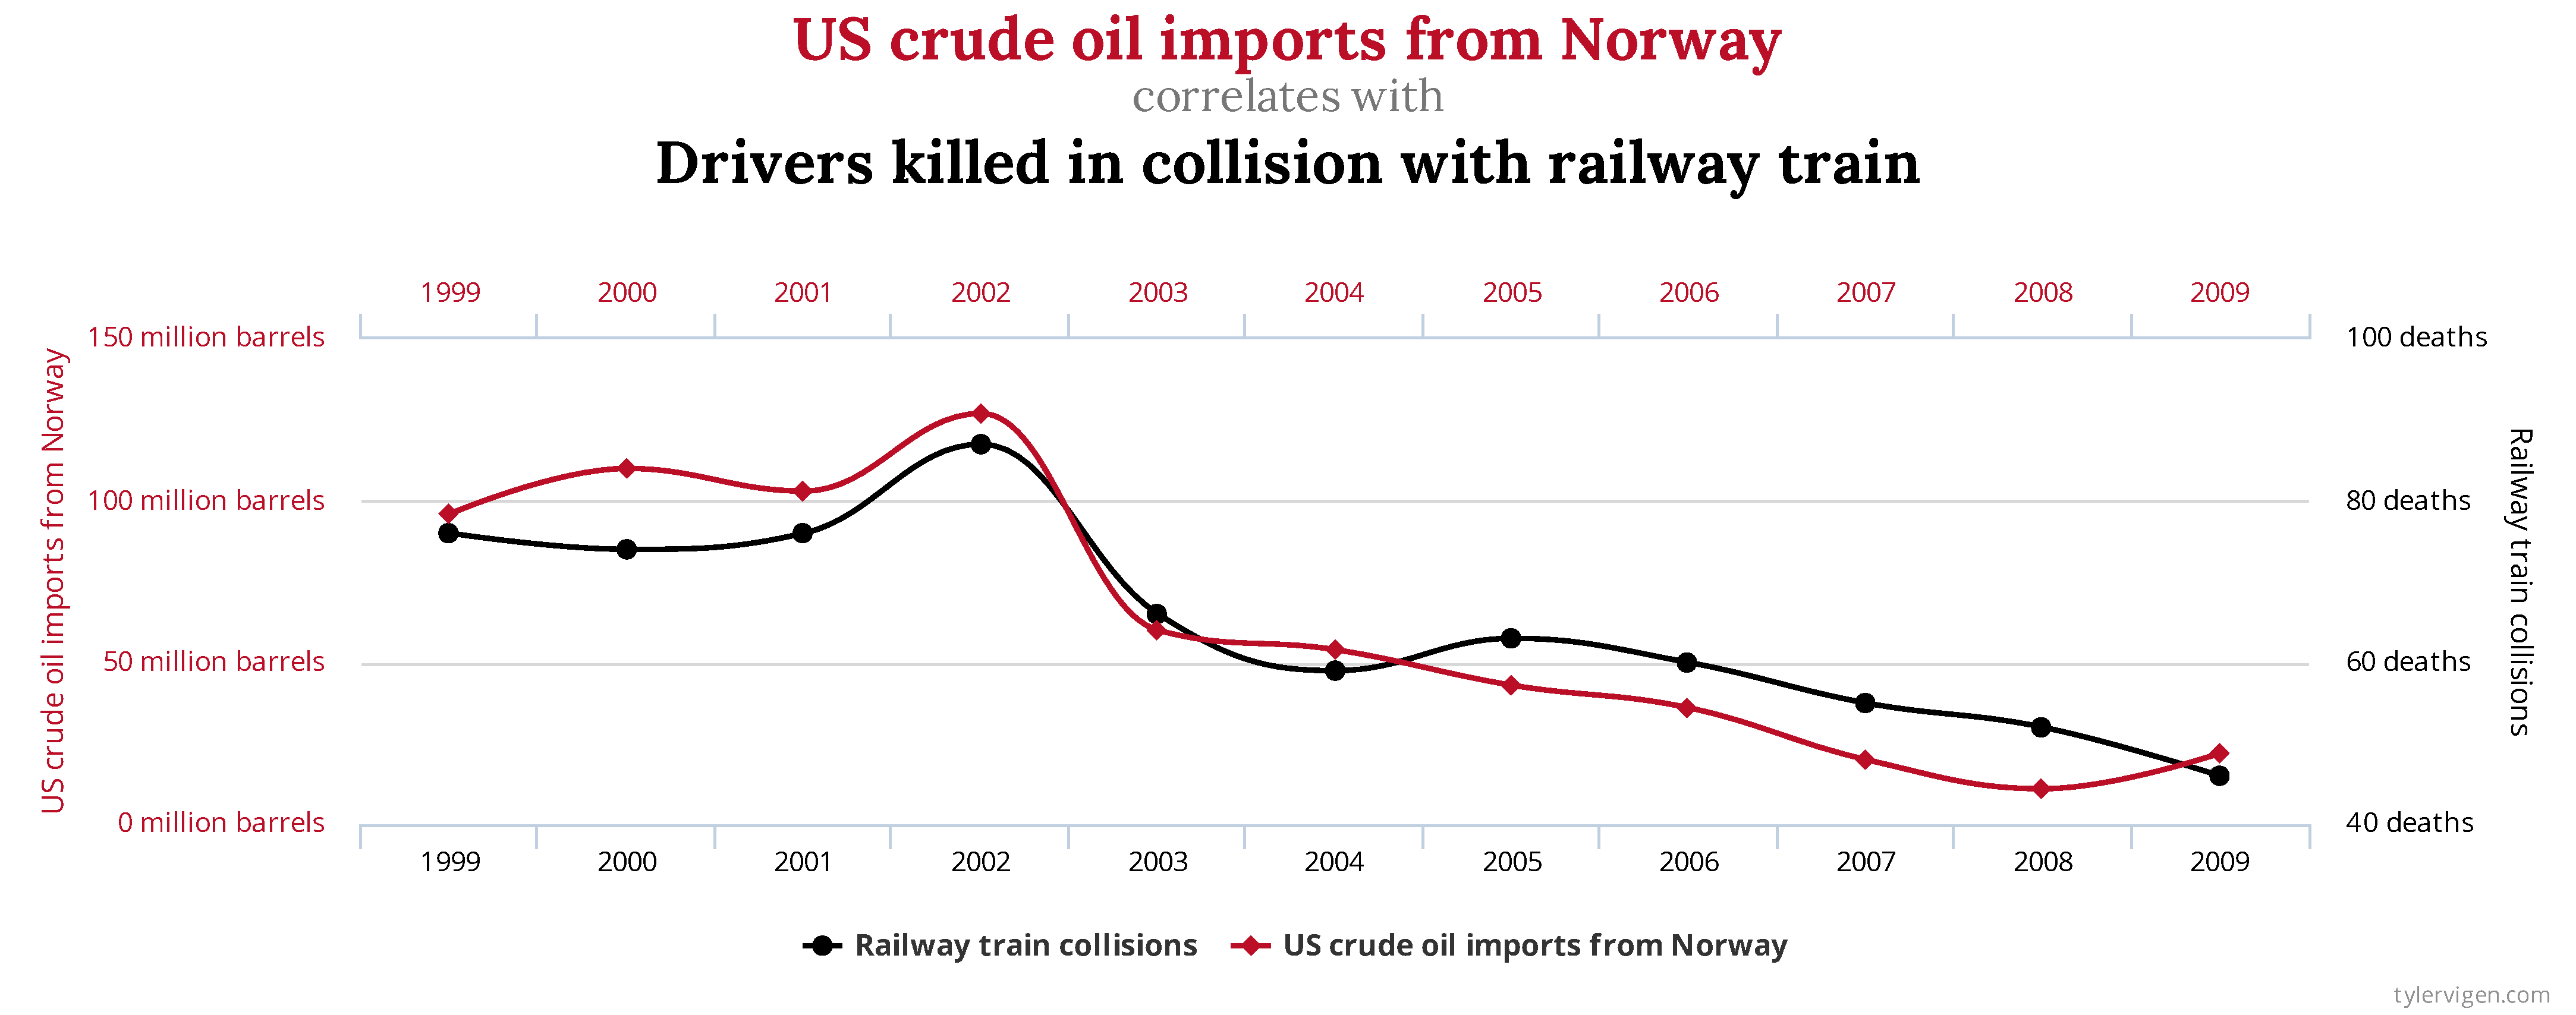
\includepdf[pages={1}]{chart_3.pdf}

\setbeamercolor{background canvas}{bg=}
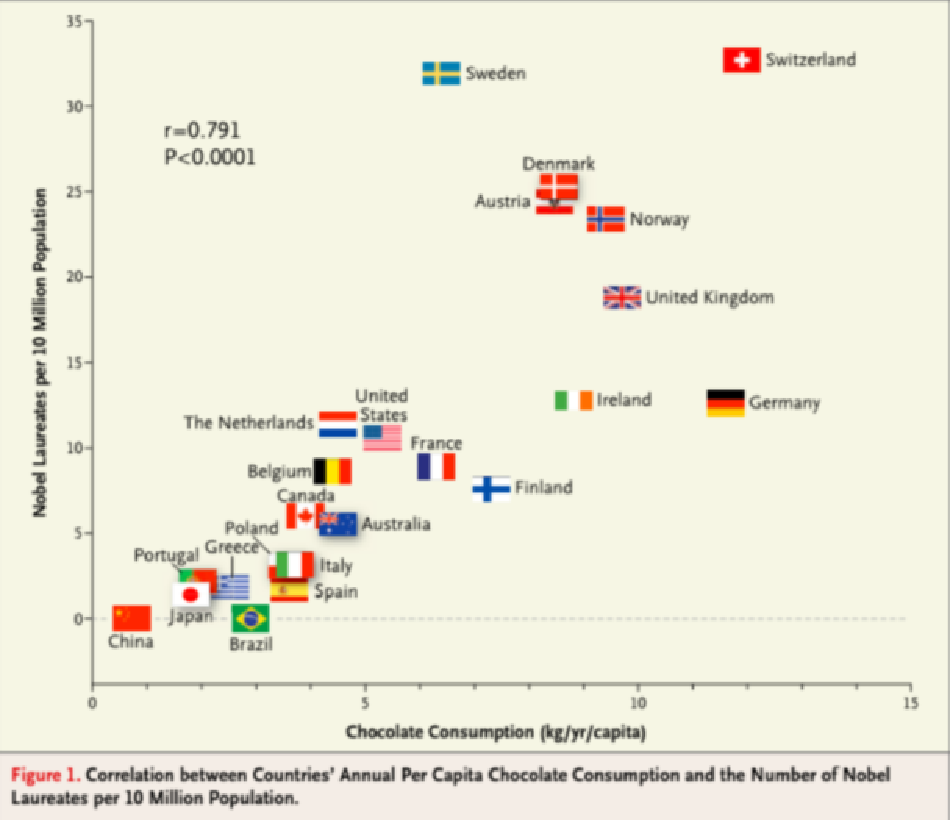
\includepdf[pages={1}]{Chocolate.pdf}

\begin{frame}
\frametitle{Learning from Data}
\begin{itemize}
\item Why isn't correlation enough?
\pause
\begin{itemize}
\item For \textbf{prediction}, correlation is fine: If we know a country has chocolate consumption of 10kg/yr/capita we can reasonably predict it will have about 25 Nobel Laureates
\pause
\item But for \textbf{intervention}, correlation does not help: forcing people to eat more chocolate does nothing on its own to produce more Nobel Laureates
\pause
\item For \textbf{explanation}, correlation also fails - it is no \textit{explanation} to say that Switzerland has the most Nobel Laureates because it has the highest chocolate consumption
\end{itemize}
\end{itemize}
\end{frame}

\section{Causal Inference}

\begin{frame}
\frametitle{Causal Inference}
\begin{itemize}
\item A focus on a single explanatory variable $D$ requires us to clearly define this 'treatment' 
\pause
\item AND to clearly define a control
\pause
\begin{itemize}
\item What is the opposite of investing \$1bn in education?
\pause
\item No investment, or investing it elsewhere?
\pause
\end{itemize}
\item Define treatment:
\end{itemize}
\[D_i = 
\begin{cases}
1 \text{, if treated} \\
0 \text{, if not treated}
\end{cases}
\]
\end{frame}

\begin{frame}
\frametitle{Causal Inference}
\begin{itemize}
\item Defining our outcome is also crucial:
\pause
\begin{itemize}
\item Can we measure our outcome of interest?
\pause
\item Is that outcome the end of the causal chain?
\pause
\item Tempting to look at many outcomes, but the risk of cherry-picking
\pause
\begin{itemize}
\item If we study 20 outcomes, on average one will show a significant effect even with no real causal effect
\end{itemize}
\end{itemize}
\end{itemize}
\end{frame}

\begin{frame}
\frametitle{Causal Inference}
\begin{itemize}
\item The \textbf{causal effect} of treatment is how each unit's outcome differs when it is treated and not treated
\pause
\item This means comparing the \textbf{Potential Outcomes} for unit $i$:
\[
Y_{Di} = 
\begin{cases}
Y_{1i}\text{   Potential Outcome if unit i treated} \\
Y_{0i}\text{   Potential Outcome if unit i NOT treated}
\end{cases}
\]
\pause
\item Individual Treatment Effect for unit $i$: $\alpha_i = Y_{1i} - Y_{0i}$
\end{itemize}
\end{frame}

\begin{frame}
\frametitle{Causal Inference}
\begin{itemize}
\item The \textbf{causal effect} of treatment is how each unit's outcome differs when it is treated and not treated
\item This means comparing the \textbf{Potential Outcomes} for unit $i$:
\[
Y_{Di} = 
\begin{cases}
Y_{1i}\text{   GDP Growth of Brazil in 2010 if a Democracy} \\
Y_{0i}\text{   GDP Growth of Brazil in 2010 if NOT a Democracy}
\end{cases}
\]
\item Individual Treatment Effect for unit $i$: $\alpha_i = Y_{1i} - Y_{0i}$
\end{itemize}
\end{frame}

\begin{frame}
\frametitle{Causal Inference}
\begin{itemize}
\item We are relying on \textbf{counterfactuals}
\pause
\begin{itemize}
\item What would have happened to the same unit if the treatment had not happened?
\pause
\item Would World War I still have happened if Archduke Franz Ferdinand had not been assassinated in 1914?
\pause
\item Would people have voted for Brexit if the campaign had been better regulated? 
\pause
\item Would Brazil have won the 2014 World Cup if Neymar had not been injured?
\pause
\end{itemize}
\end{itemize}
\end{frame}

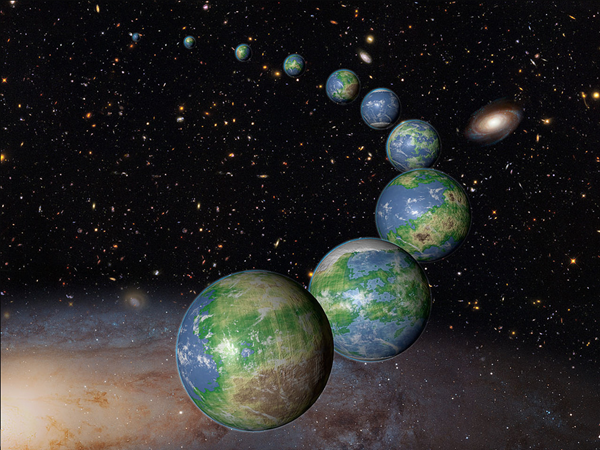
\includegraphics[width=1\textwidth]{figure/Multiverse.png}

\begin{frame}
\frametitle{Causal Inference}
\footnotesize
\begin{table}[htbp]
  \centering
  \caption{Potential Outcomes are just another Variable for each Unit}
    \begin{tabular}{|p{2.4cm}|p{2.4cm}|p{2.4cm}|p{2.4cm}|}
    \hline
          & \multicolumn{1}{p{2.4cm}|}{GDP Growth if Democracy} & \multicolumn{1}{p{2.4cm}|}{GDP Growth if  NOT Democracy} &  Treatment Effect\bigstrut\\
    \hline
          & \multicolumn{1}{l|}{$Y_1$} & \multicolumn{1}{l|}{$Y_0$} & \multicolumn{1}{l|}{$Y_1-Y_0$} \bigstrut\\
    \hline
    Brasil & 6     & 3     & 3 \bigstrut\\
    \hline
    Argentina & 8    & 5     & 3 \bigstrut\\
    \hline
    Uruguay & 3 & 3 & 0  \bigstrut\\
    \hline
    Bolivia & 0     & 2     & -2 \bigstrut\\
    \hline
    Colombia & 4    & 4    & 0 \bigstrut\\
    \hline
    Peru & 4     & 2     & 2 \bigstrut\\
    \hline
    \end{tabular}%
  \label{tab:addlabel}%
\end{table}%
\normalsize
\end{frame}

\begin{frame}
\frametitle{Causal Inference}
\begin{itemize}
\item Political Science is not about explaining individual events
\pause
\item We ideally want general theories that apply to \textit{all our units}
\pause
\item To explain a systematic treatment - not a single event - we need \textbf{multiple counterfactual comparisons}
\pause
\item We know how democracy works in Europe; the question is what will happen if it becomes more common in the whole world?
\pause
\begin{block}{Average Treatment Effect}
\item We want to calculate an \textbf{Average Treatment Effect} 
\pause 
\item $$ATE=E(\alpha_i) = E (Y_1 - Y_0) = E(Y_1) - E(Y_0) = \frac{\sum_i (Y_{1i} - Y_{0i})}{N}$$
\end{block}
\end{itemize}
\end{frame}

\begin{frame}
\frametitle{Causal Inference}
\footnotesize
\begin{table}[htbp]
  \centering
  \caption{Potential Outcomes are just another Variable for each Unit}
    \begin{tabular}{|p{2.4cm}|p{2.4cm}|p{2.4cm}|p{2.4cm}|}
    \hline
          & \multicolumn{1}{p{2.4cm}|}{GDP Growth if Democracy} & \multicolumn{1}{p{2.4cm}|}{GDP Growth if  NOT Democracy} & Treatment Effect \bigstrut\\
    \hline
          & \multicolumn{1}{p{2.4cm}|}{$Y_1$} & \multicolumn{1}{l|}{$Y_0$} & \multicolumn{1}{l|}{$Y_{1} - Y_{0}$} \bigstrut\\
    \hline
    Brasil & 6     & 3     & 3 \bigstrut\\
    \hline
    Argentina & 8    & 5     & 3 \bigstrut\\
    \hline
    Uruguay & 3 & 3 & 0  \bigstrut\\
    \hline
    Bolivia & 0     & 2     & -2 \bigstrut\\
    \hline
    Colombia & 4    & 4    & 0 \bigstrut\\
    \hline
    Peru & 4     & 2     & 2 \bigstrut\\
    \hline
    \textbf{Average Treatment Effect} & \textbf{4.17} & \textbf{3.17} & \textbf{1} \bigstrut\\
    \hline
    \end{tabular}%
  \label{tab:addlabel}%
\end{table}%
\normalsize
\end{frame}

\begin{frame}
\frametitle{Causal Inference}
\begin{block}{The Fundamental Problem of Causal Inference}
\begin{itemize}
\item No units can receive \textbf{both} treatment and control
\pause
\item So we can never observe both $Y_1$ and $Y_0$ \textbf{for the same unit}
\pause
\item \textit{Individual} Treatment Effects are \textbf{Impossible to Estimate}
\end{itemize}
\end{block}
\pause
\[
Y_{i}^{obs} = 
\begin{cases}
Y_{1i} \text{ if } D_i=1 \\
Y_{0i} \text{ if } D_i=0
\end{cases}
\]
\pause
$$Y_{i}^{obs} = D_i \cdot Y_{1i} + (1-D_i) \cdot Y_{0i}$$
\end{frame}


\begin{frame}
\frametitle{Causal Inference}
\footnotesize
\begin{table}[htbp]
  \centering
  \caption{Potential Outcomes Example}
    \begin{tabular}{|p{1.8cm}|p{1.8cm}|p{2cm}|p{2cm}|p{2cm}|}
    \hline
          & \multicolumn{1}{p{1.8cm}|}{Democracy?} & \multicolumn{1}{p{2cm}|}{GDP Growth if Democracy} & \multicolumn{1}{p{2.2cm}|}{GDP Growth if NOT Democracy} & Treatment Effect \bigstrut\\
    \hline
          & \multicolumn{1}{p{1.8cm}|}{$D_i$} & \multicolumn{1}{p{2cm}|}{$Y_1$} & \multicolumn{1}{p{2.2cm}|}{$Y_0$} & \multicolumn{1}{p{1.8cm}|}{$Y_{1} - Y_{0}$} \bigstrut\\
    \hline
    Brasil & 0 & ?     & 3     & ? \bigstrut\\
    \hline
    Argentina & 0 & ?    & 5     & ? \bigstrut\\
    \hline
    Uruguay & 0 & ? & 3 & ?  \bigstrut\\
    \hline
    Bolivia & 1  & 0     & ?     & ? \bigstrut\\
    \hline
    Colombia & 1  & 4    & ?    & ? \bigstrut\\
    \hline
    Peru & 0 & ?     & 2     & ? \bigstrut\\
\hline
    \end{tabular}%
  \label{tab:addlabel}%
\end{table}%
\normalsize
\end{frame}

\begin{frame}
\frametitle{Causal Inference}
\footnotesize
\begin{table}[htbp]
  \centering
  \caption{Potential Outcomes Example}
    \begin{tabular}{|p{1.8cm}|p{1.8cm}|p{2cm}|}
    \hline
          & \multicolumn{1}{p{1.8cm}|}{Democracy?} & \textbf{Observed} GDP Growth \bigstrut\\
    \hline
          & \multicolumn{1}{p{1.8cm}|}{$D_i$} & \multicolumn{1}{p{1.8cm}|}{$Y^{obs}$} \bigstrut\\
    \hline
    Brasil & 0 & 3 \bigstrut\\
    \hline
    Argentina & 0      & 5 \bigstrut\\
    \hline
    Uruguay & 0 & 3  \bigstrut\\
    \hline
    Bolivia & 1      & 0 \bigstrut\\
    \hline
    Colombia & 1    & 4 \bigstrut\\
    \hline
    Peru & 0 & 2 \bigstrut\\
    \hline
    \end{tabular}%
  \label{tab:addlabel}%
\end{table}%
\normalsize
\end{frame}

\begin{frame}
\frametitle{Causal Inference}
\begin{itemize}
\item Actually, nothing stops us calculating the \textbf{Average Treatment Effect}
\pause
\item The question is, is the ATE accurate?
\pause
\end{itemize}
\scriptsize
\begin{table}[htbp]
  \centering
    \begin{tabular}{|p{1.8cm}|p{1.8cm}|p{2cm}|p{2cm}|p{2cm}|}
    \hline
          & \multicolumn{1}{p{1.8cm}|}{Democracy?} & \multicolumn{1}{p{2cm}|}{GDP Growth if Democracy} & \multicolumn{1}{p{2.2cm}|}{GDP Growth if NOT Democracy} & \textbf{Treatment Effect} \bigstrut\\
    \hline
          & \multicolumn{1}{p{1.8cm}|}{$D_i$} & \multicolumn{1}{p{2cm}|}{$Y_1$} & \multicolumn{1}{p{2.2cm}|}{$Y_0$} & \multicolumn{1}{p{1.8cm}|}{$Y_{1} - Y_{0}$} \bigstrut\\
    \hline
    Brasil & 0 & 6     & 3     & 3 \bigstrut\\
    \hline
    Argentina & 0 & 8    & 5     & 3 \bigstrut\\
    \hline
    Uruguay & 0 & 3 & 3 & 0  \bigstrut\\
    \hline
    Bolivia & 1 & 0     & 2     & -2 \bigstrut\\
    \hline
    Colombia & 1 & 4    & 4    & 0 \bigstrut\\
    \hline
    Peru & 0 & 4     & 2     & 2 \bigstrut\\
    \hline
    \textbf{Average Treatment Effect} & & \textbf{4.17} & \textbf{3.17} & \textbf{1} \bigstrut\\
    \hline
    \end{tabular}%
  \label{tab:addlabel}%
\end{table}%
\normalsize
\end{frame}

\begin{frame}
\frametitle{Causal Inference}
\begin{itemize}
\item Actually, nothing stops us calculating the \textbf{Average Treatment Effect}
\item The question is, is the ATE accurate?
\end{itemize}
\scriptsize
\begin{table}[htbp]
  \centering
    \begin{tabular}{|p{1.8cm}|p{1.8cm}|p{2cm}|p{2cm}|p{2cm}|}
    \hline
          & \multicolumn{1}{p{1.8cm}|}{Democracy?} & \multicolumn{1}{p{2cm}|}{GDP Growth if Democracy} & \multicolumn{1}{p{2.2cm}|}{GDP Growth if NOT Democracy} & \textbf{Treatment Effect} \bigstrut\\
    \hline
          & \multicolumn{1}{p{1.8cm}|}{$D_i$} & \multicolumn{1}{p{2cm}|}{$Y_1$} & \multicolumn{1}{p{2.2cm}|}{$Y_0$} & \multicolumn{1}{p{1.8cm}|}{$Y_{1} - Y_{0}$} \bigstrut\\
    \hline
    Brasil & 0 & ?     & 3     & ? \bigstrut\\
    \hline
    Argentina & 0 & ?    & 5     & ? \bigstrut\\
    \hline
    Uruguay & 0 & ? & 3 & ?  \bigstrut\\
    \hline
    Bolivia & 1 & 0     & ?     & ? \bigstrut\\
    \hline
    Colombia & 1 & 4    & ?    & ? \bigstrut\\
    \hline
    Peru & 0 & ?     & 2     & ? \bigstrut\\
    \hline
    \textbf{Average Treatment Effect} & & \textbf{2} & \textbf{3.25} & \textbf{-1.25} \bigstrut\\
    \hline
    \end{tabular}%
  \label{tab:addlabel}%
\end{table}%
\normalsize
\end{frame}

\begin{frame}
\frametitle{Causal Inference}
\begin{itemize}
\item \textbf{So what went wrong?}
\pause
\item The potential outcomes we \textbf{observe} are a \textbf{biased representation} of the potential outcomes of all the units
\pause
\end{itemize}
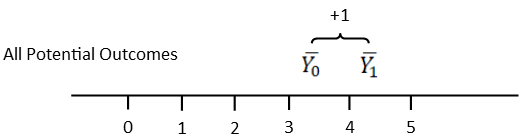
\includegraphics[width=0.9\textwidth]{figure/PO_number_line_1.png}
\end{frame}

\begin{frame}
\frametitle{Causal Inference}
\begin{itemize}
\item \textbf{So what went wrong?}
\item The potential outcomes we \textbf{observe} are a \textbf{biased representation} of the potential outcomes of all the units
\end{itemize}
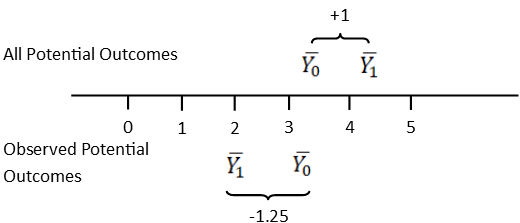
\includegraphics[width=0.9\textwidth]{figure/PO_number_line_2.png}
\begin{itemize}
\item $E(Y_1)$ values are \textbf{biased lower} in the observed data
\pause
\item $E(Y_0)$ values are \textbf{biased higher} in the observed data
\pause
\item So $E(Y_1)-E(Y_0)$ is \textbf{biased}
\end{itemize}
\end{frame}

\begin{frame}
\frametitle{Causal Inference}
\begin{itemize}
\item The Fundamental Problem of Causal Inference means we can only discover causal relationships by comparing \textbf{across units}
\pause
\item Comparing treated $i$ and control $j$ units
\pause
\item If potential outcomes are biased in our observed data:
\pause
\begin{itemize}
\item Our \textbf{counterfactual case $j$} does not represent what would have happened to $i$ in the absence of treatment
\pause
\item Counterfactuals are not \textbf{plausible}
\pause
\item Causal effects are \textbf{biased}
\end{itemize}
\end{itemize}
\end{frame}

\begin{frame}
\frametitle{Causal Inference}
\begin{knitrout}
\definecolor{shadecolor}{rgb}{0.969, 0.969, 0.969}\color{fgcolor}
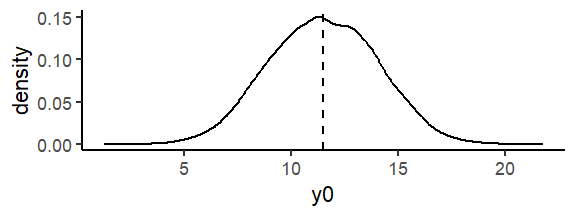
\includegraphics[width=\maxwidth]{figure/OVB1a-1} 
\end{knitrout}
\pause
\begin{knitrout}
\definecolor{shadecolor}{rgb}{0.969, 0.969, 0.969}\color{fgcolor}
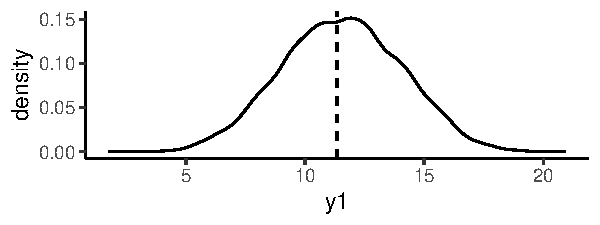
\includegraphics[width=\maxwidth]{figure/OVB2a-1} 
\end{knitrout}
\end{frame}

\begin{frame}
\frametitle{Causal Inference}
\begin{knitrout}
\definecolor{shadecolor}{rgb}{0.969, 0.969, 0.969}\color{fgcolor}
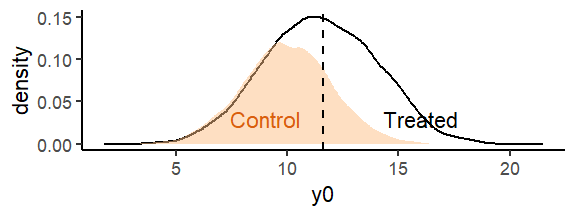
\includegraphics[width=\maxwidth]{figure/OVB1b-1} 
\end{knitrout}

\begin{knitrout}
\definecolor{shadecolor}{rgb}{0.969, 0.969, 0.969}\color{fgcolor}
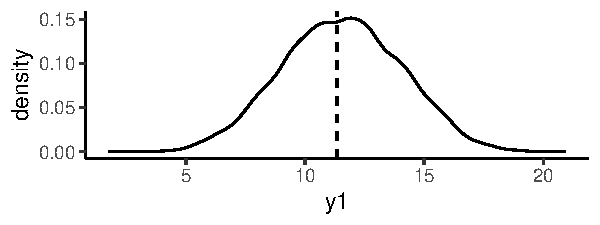
\includegraphics[width=\maxwidth]{figure/OVB2b-1} 
\end{knitrout}
\end{frame}

\begin{frame}
\frametitle{Causal Inference}
\begin{knitrout}
\definecolor{shadecolor}{rgb}{0.969, 0.969, 0.969}\color{fgcolor}
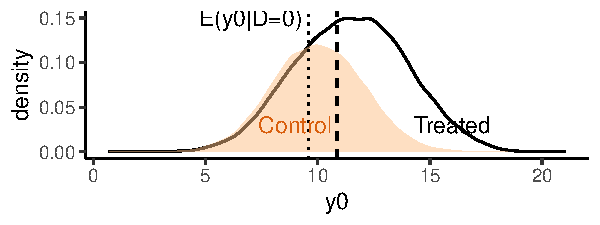
\includegraphics[width=\maxwidth]{figure/OVB1c-1} 
\end{knitrout}

\begin{knitrout}
\definecolor{shadecolor}{rgb}{0.969, 0.969, 0.969}\color{fgcolor}
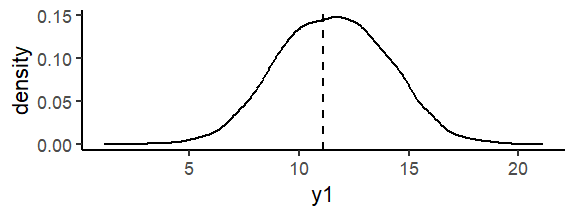
\includegraphics[width=\maxwidth]{figure/OVB2c-1} 
\end{knitrout}
\end{frame}

\begin{frame}
\frametitle{Causal Inference}
\begin{knitrout}
\definecolor{shadecolor}{rgb}{0.969, 0.969, 0.969}\color{fgcolor}
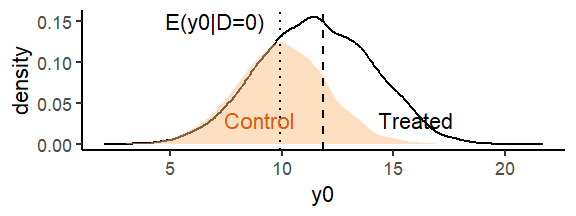
\includegraphics[width=\maxwidth]{figure/OVB1d-1} 
\end{knitrout}

\begin{knitrout}
\definecolor{shadecolor}{rgb}{0.969, 0.969, 0.969}\color{fgcolor}
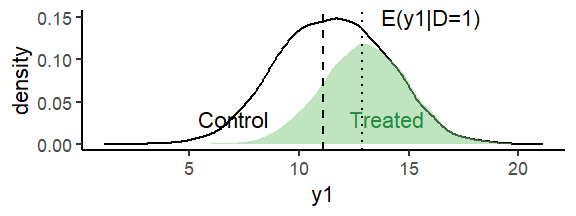
\includegraphics[width=\maxwidth]{figure/OVB2d-1} 
\end{knitrout}
\end{frame}

\begin{frame}
\frametitle{Causal Inference}
\begin{itemize}
\item Lots of averages:
\end{itemize}
\begin{table}[htbp]
  \centering
    \begin{tabular}{|c|l|l|l|}
    \hline
          &       & \multicolumn{2}{c|}{Hypothetical outcome} \bigstrut\\
    \hline
          &       & $Y0$    & $Y1$ \bigstrut\\
    \hline
    \multirow{2}[4]{*}{Actual Treatment} & $D=0$   & $E(Y_{0i}|D=0)$ & $E(Y_{1i}|D=0)$ \bigstrut\\
\cline{2-4}          & $D=1$   & $E(Y_{0i}|D=1)$ & $E(Y_{1i}|D=1)$ \bigstrut\\
    \hline
    \end{tabular}%
  \label{tab:addlabel}%
\end{table}%
\end{frame}

\begin{frame}
\frametitle{Causal Inference}
\begin{itemize}
\item Lots of averages:
\end{itemize}
\begin{table}[htbp]
  \centering
    \begin{tabular}{|c|l|l|l|}
    \hline
          &       & \multicolumn{2}{c|}{Hypothetical outcome} \bigstrut\\
    \hline
          &       & $Y0$    & $Y1$ \bigstrut\\
    \hline
    \multirow{2}[4]{*}{Actual Treatment} & $D=0$   & \cellcolor{blue!25}$E(Y_{0i}|D=0)$ & $E(Y_{1i}|D=0)$ \bigstrut\\
\cline{2-4}          & $D=1$   & $E(Y_{0i}|D=1)$ & \cellcolor{blue!25}$E(Y_{1i}|D=1)$ \bigstrut\\
    \hline
    \end{tabular}%
  \label{tab:addlabel}%
\end{table}%
\end{frame}

\section{Treatment Assignment}

\begin{frame}
\frametitle{Treatment Assignment Mechanism}
\begin{itemize}
\item The comparability of treatment and control units depends on \textit{how} they got to be treated
\pause
\begin{itemize}
\item On the \textbf{Treatment Assignment Mechanism}
\pause
\end{itemize}
\item If we 'treated' an outlier like the Galapagos Islands, could we find a comparable control unit?
\pause
\item Comparisons are 'better' where the \textbf{Treatment Assignment Mechanism is independent of potential outcomes}
\pause
\begin{itemize}
\item I.e. Whether you got treatment had \textbf{nothing} to do with how much you would benefit from treatment 
\item This makes it more likely that potential outcomes are 'balanced'
\end{itemize}
\end{itemize}
\end{frame}

\begin{frame}
\frametitle{Treatment Assignment Mechanism}
\begin{itemize}
\item A 'real-world' treatment assignment is \textit{highly unlikely} to create comparable potential outcomes
\pause
\item And we do not know what the treatment assignment mechanism was
\begin{itemize}
\item Because we did not control treatment assignment ourselves
\pause
\end{itemize}
\pause
\item So we do not know which units might be appropriate counterfactuals
\end{itemize}
\end{frame}


\begin{frame}
\frametitle{Exercise}
\begin{itemize}
\item Does fruit make you happier? 
\pause
\begin{itemize}
\item Write down on a piece of paper a number between 0 and 10 representing how happy you would be if I gave you an apple now. 
\pause
\item Label this number $Y_1$.
\pause
\item Then write down a second number between 0 and 10 representing how happy you would be if I did NOT give you an apple now. 
\pause
\item Label this number $Y_0$.
\pause
\end{itemize}
\item These are your \textbf{potential outcomes}.
\end{itemize}
\end{frame}

\begin{frame}
\frametitle{Exercise}
\begin{itemize}
\item Now we will consider how estimates of the average effect of fruit on happiness vary depending on how treatment (apples) are assigned.
\pause
\begin{enumerate}
\item All the female participants are given an apple.
\pause
\item The tallest half are given an apple.
\pause
\item You are free to choose yourself to take an apple or not.
\pause
\item Apples are distributed randomly
\end{enumerate}
\end{itemize}
\end{frame}

\begin{frame}
\frametitle{Treatment Assignment Mechanism}
\begin{itemize}
\item Explanation is more reliable where the \textbf{Treatment Assignment Mechanism is Independent of Potential Outcomes}
\pause
\begin{itemize}
\item Independent means the values of the potential outcomes give us no information about whether that unit was treated
\pause
\item Potential outcomes are 'balanced' across control and treatment groups
\pause
\end{itemize}
\end{itemize}
\begin{block}{Independence of Treatment Assignment}
\begin{itemize}
\item Treatment Assignment does NOT depend on the values of units' Potential Outcomes
\pause 
\item $(Y_1,Y_0) \perp D$
\pause
\item $Pr(D|(Y_1,Y_0)) = Pr(D)$
\pause
\item $E(Y|D=1) = E(Y|D=0) = E(Y)$
\end{itemize}
\end{block}
\end{frame}

\section{3 Critiques}

\begin{frame}
\frametitle{3 Critiques}
\begin{itemize}
\item Why are potential outcomes biased in our data?
\pause
\begin{enumerate}
\item Omitted Variables
\pause
\item Reverse Causation
\pause
\item Selection Bias
\pause
\end{enumerate}
\item In all of these cases \textbf{the potential outcomes are distorted}
\pause
\item So basic regression is \textbf{biased}
\end{itemize}
\end{frame}

\begin{frame}
\frametitle{Omitted Variable Bias}
\begin{multicols}{2}
A real causal relationship:
\begin{knitrout}
\definecolor{shadecolor}{rgb}{0.969, 0.969, 0.969}\color{fgcolor}
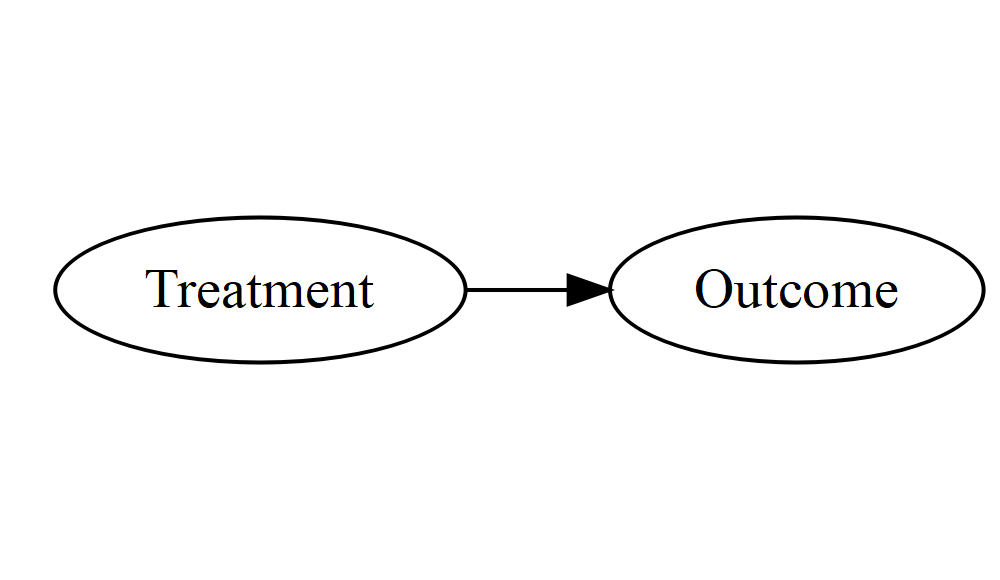
\includegraphics[width=\maxwidth]{figure/explanation3-1} 
\end{knitrout}

\columnbreak

\pause
Being misled by omitted variable bias:
\begin{knitrout}
\definecolor{shadecolor}{rgb}{0.969, 0.969, 0.969}\color{fgcolor}
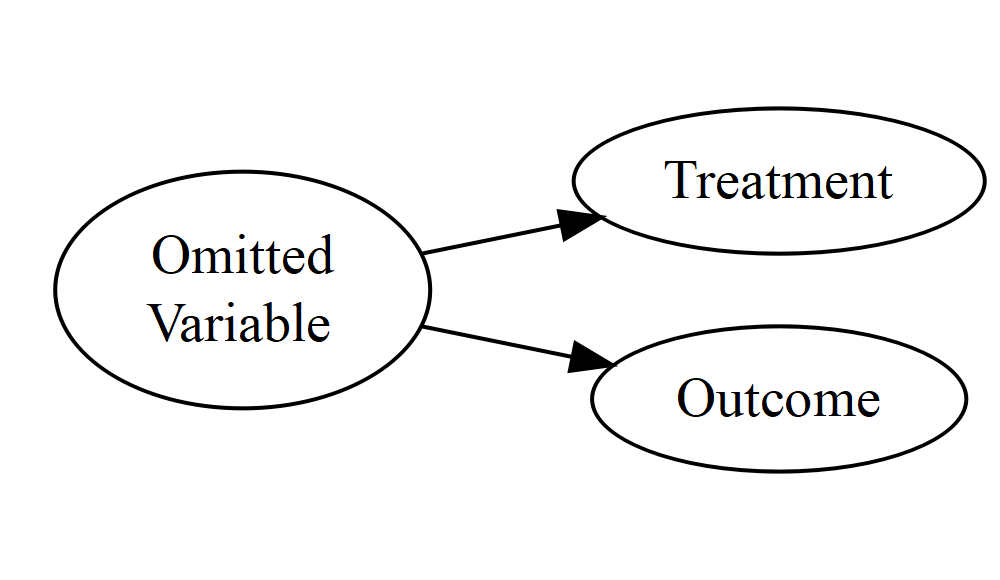
\includegraphics[width=\maxwidth]{figure/explanation4-1} 
\end{knitrout}
\end{multicols}
\begin{itemize}
\pause
\item A third variable causes some units to have \textbf{different values of potential outcomes}, AND for those \textbf{same units to be treated}
\pause
\item So treated units have non-representative $Y_1$
\pause
\item And control units have non-representative $Y_0$
\end{itemize}
\end{frame}

\begin{frame}
\frametitle{Omitted Variable Bias}
\begin{multicols}{2}
A real causal relationship:
\begin{knitrout}
\definecolor{shadecolor}{rgb}{0.969, 0.969, 0.969}\color{fgcolor}
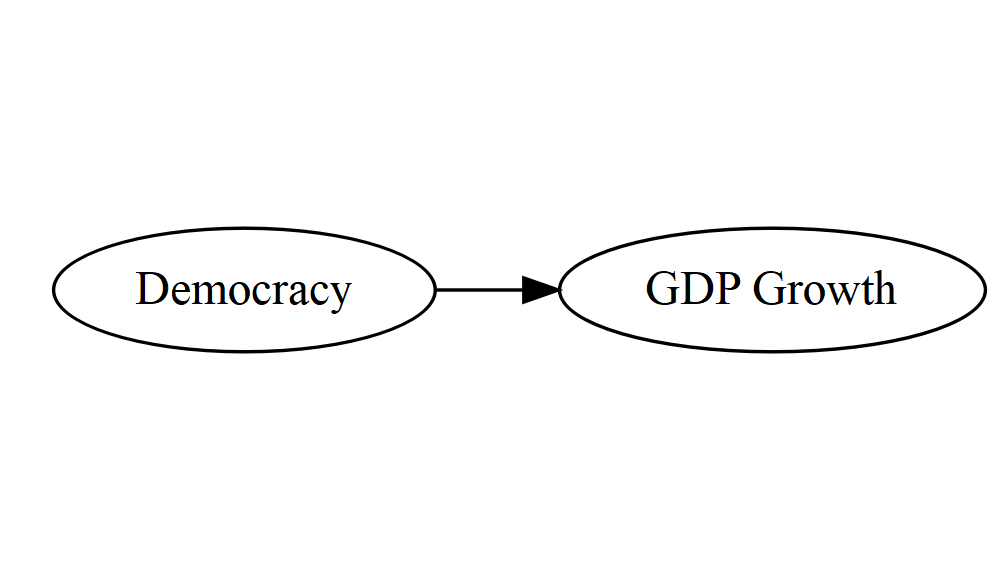
\includegraphics[width=\maxwidth]{figure/explanation9-1} 
\end{knitrout}
\columnbreak
Being misled by omitted variable bias:
\begin{knitrout}
\definecolor{shadecolor}{rgb}{0.969, 0.969, 0.969}\color{fgcolor}
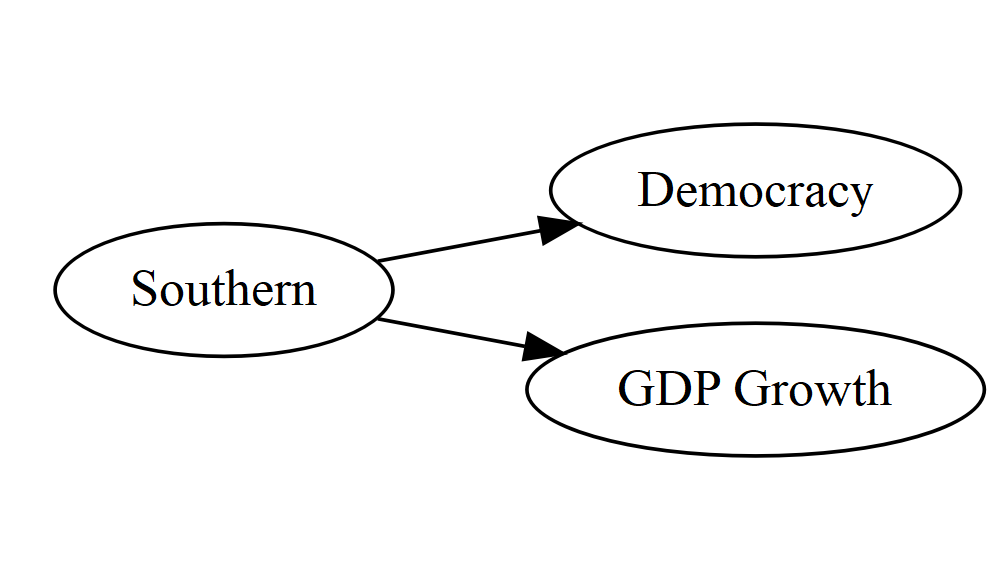
\includegraphics[width=\maxwidth]{figure/explanation10-1} 
\end{knitrout}
\end{multicols}
\begin{itemize}
\pause
\item Southern Cone countries faced conditions that encouraged both democracy and rapid GDP growth
\end{itemize}
\end{frame}

\begin{frame}
\frametitle{Omitted Variable Bias}
\begin{knitrout}
\definecolor{shadecolor}{rgb}{0.969, 0.969, 0.969}\color{fgcolor}
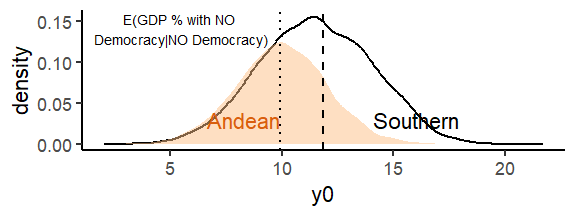
\includegraphics[width=\maxwidth]{figure/OVB3-1} 
\end{knitrout}

\begin{knitrout}
\definecolor{shadecolor}{rgb}{0.969, 0.969, 0.969}\color{fgcolor}
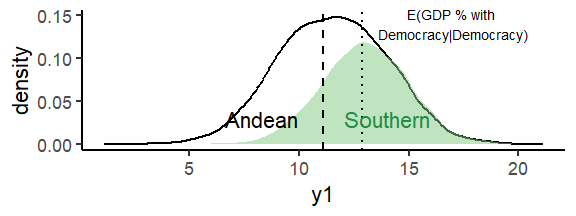
\includegraphics[width=\maxwidth]{figure/OVB4-1} 
\end{knitrout}
\end{frame}

\begin{frame}
\frametitle{Omitted Variable Bias}
\scriptsize
\begin{table}[htbp]
  \centering
    \begin{tabular}{|p{1.6cm}|p{1.6cm}|p{1.6cm}|p{1.6cm}|p{1.6cm}|p{1.6cm}|}
    \hline
           & \multicolumn{1}{|p{1.6cm}|}{Andean?} & \multicolumn{1}{|p{1.6cm}|}{Democracy?} & \multicolumn{1}{p{1.6cm}|}{GDP Growth if Dem} & \multicolumn{1}{p{1.6cm}|}{GDP Growth if NOT Dem} & \textbf{Treatment Effect} \bigstrut\\
    \hline
          & \multicolumn{1}{|p{1.6cm}|}{$X_i$} & \multicolumn{1}{p{1.6cm}|}{$D_i$} & \multicolumn{1}{p{1.6cm}|}{$Y_1$} & \multicolumn{1}{p{1.6cm}|}{$Y_0$} & \multicolumn{1}{p{1.6cm}|}{$Y_{1} - Y_{0}$} \bigstrut\\
    \hline
    Brasil & 1 & 1 & 6     & ?     & ? \bigstrut\\
    \hline
    Argentina & 1 & 1 & 8    & ?     & ? \bigstrut\\
    \hline
    Uruguay & 1 & 1 & 3 & ? & ?  \bigstrut\\
    \hline
    Bolivia & 0 & 0 & ?     & 2     & ? \bigstrut\\
    \hline
    Colombia & 0 & 0 & ?    & 4    & ? \bigstrut\\
    \hline
    Peru & 0 & 0 & ?     & 2     & ? \bigstrut\\
    \hline
    \textbf{Average Treatment Effect}& & & \textbf{5.7} & \textbf{2.7} & \textbf{3} \bigstrut\\
    \hline
    \end{tabular}%
  \label{tab:addlabel}%
\end{table}%
\normalsize
\end{frame}

\begin{frame}
\frametitle{Omitted Variable Bias}
\begin{knitrout}
\definecolor{shadecolor}{rgb}{0.969, 0.969, 0.969}\color{fgcolor}
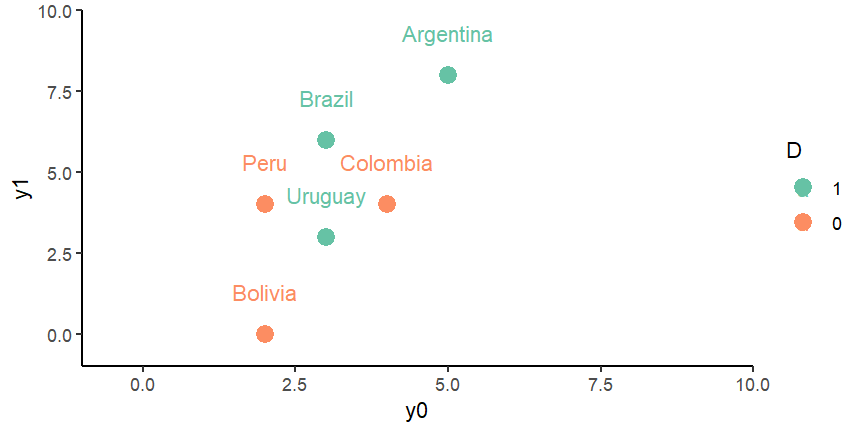
\includegraphics[width=\maxwidth]{figure/Chart_1-1} 
\end{knitrout}
\end{frame}

\begin{frame}
\frametitle{Omitted Variable Bias}
\begin{knitrout}
\definecolor{shadecolor}{rgb}{0.969, 0.969, 0.969}\color{fgcolor}
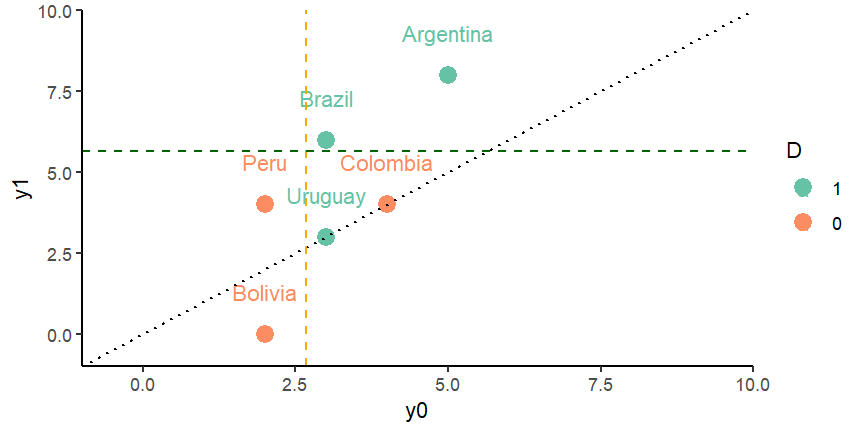
\includegraphics[width=\maxwidth]{figure/Chart_1b-1} 
\end{knitrout}
\begin{itemize}
\item $E(Y_1|D=1) - E(Y_0|D=0) = 5.7 - 2.7 = 3$
\end{itemize}
\end{frame}

\begin{frame}
\frametitle{Omitted Variable Bias}
\begin{itemize}
\item Let's say that $Y_{1i} = Y_{0i} + \alpha$, where $\alpha$ is the real constant treatment effect
\end{itemize}
$$ \hat{ATE} = E(Y_1|D=1) - E(Y_0|D=0)$$ \\ \pause
$$ \hat{ATE} = \underbrace{\alpha}_\text{Real ATE} + \underbrace{E(Y_0|D=1) - E(Y_0|D=0)}_\text{Bias}$$ \\
\end{frame}


\begin{frame}
\frametitle{Reverse Causation}
\begin{multicols}{2}
A real causal relationship:
\begin{knitrout}
\definecolor{shadecolor}{rgb}{0.969, 0.969, 0.969}\color{fgcolor}
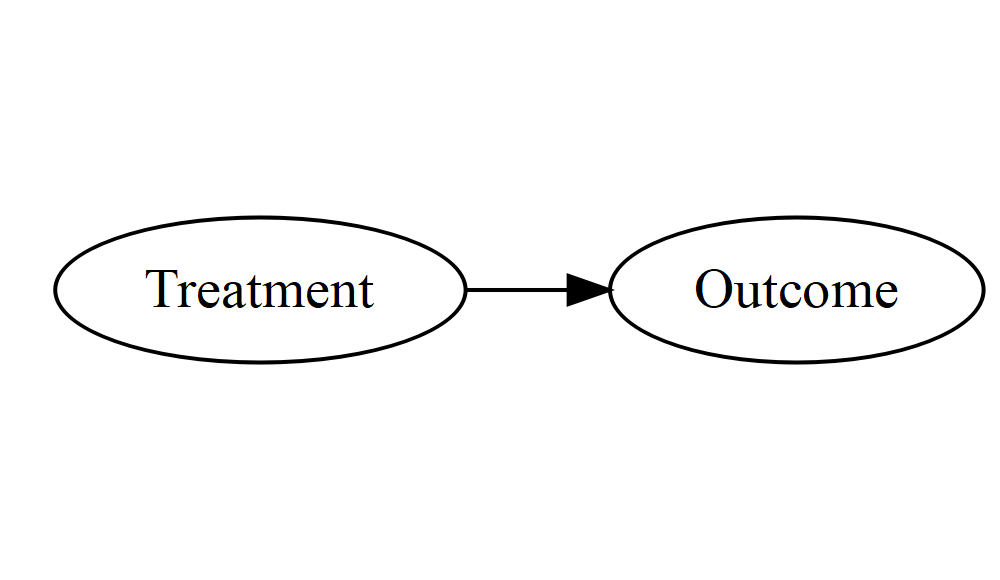
\includegraphics[width=\maxwidth]{figure/explanation5-1} 
\end{knitrout}
\columnbreak
\pause
Being misled by reverse causation:
\begin{knitrout}
\definecolor{shadecolor}{rgb}{0.969, 0.969, 0.969}\color{fgcolor}
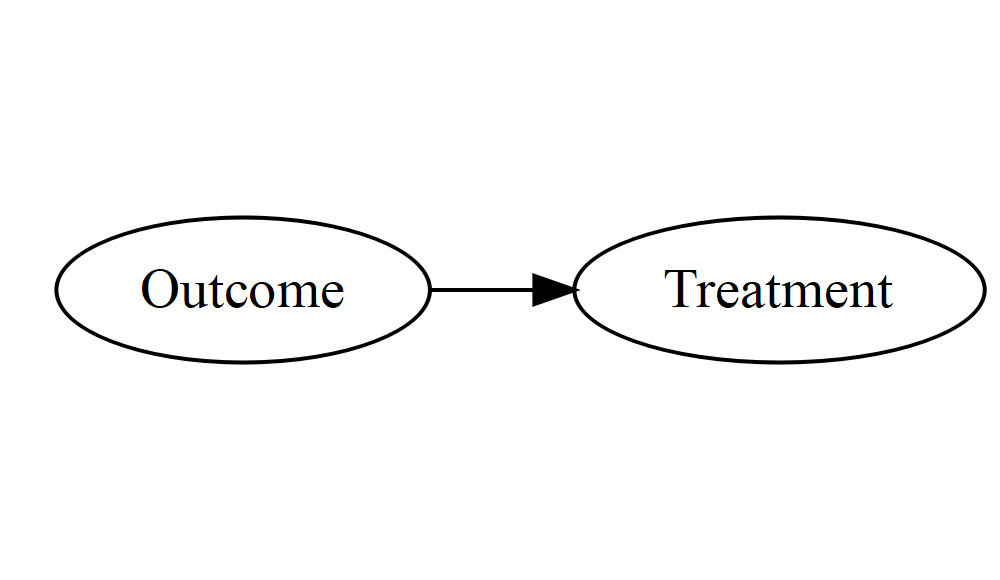
\includegraphics[width=\maxwidth]{figure/explanation6-1} 
\end{knitrout}
\end{multicols}
\begin{itemize}
\pause
\item $D$ does not affect $Y$, but higher $Y$ makes treatment ($D$) more likely
\pause
\item So the two variables are \textbf{correlated}
\end{itemize}
\end{frame}

\begin{frame}
\frametitle{Reverse Causation}
\begin{multicols}{2}
A real causal relationship:
\begin{knitrout}
\definecolor{shadecolor}{rgb}{0.969, 0.969, 0.969}\color{fgcolor}
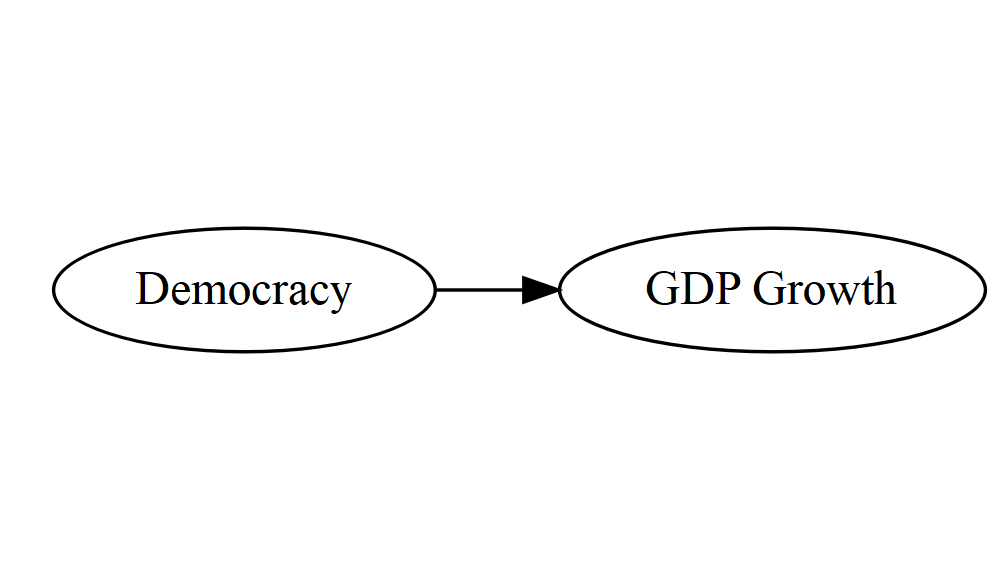
\includegraphics[width=\maxwidth]{figure/reverse1-1} 
\end{knitrout}
\columnbreak
Being misled by reverse causation:
\begin{knitrout}
\definecolor{shadecolor}{rgb}{0.969, 0.969, 0.969}\color{fgcolor}
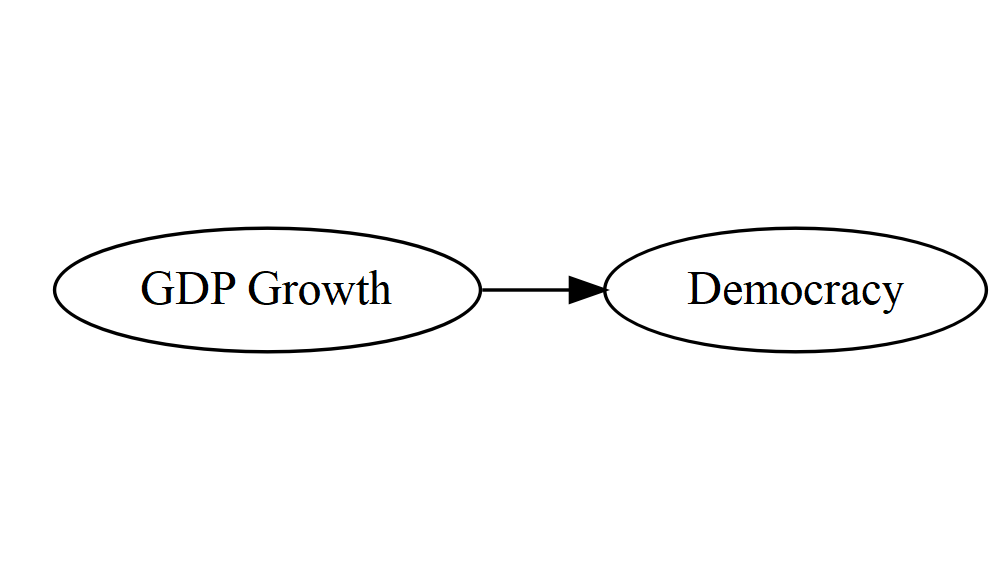
\includegraphics[width=\maxwidth]{figure/reverse2-1} 
\end{knitrout}
\end{multicols}
\begin{itemize}
\pause
\item GDP Growth encourages democratization
\pause
\item So democracies are more likely to have experienced high growth rates
\end{itemize}
\end{frame}

\begin{frame}
\frametitle{Reverse Causation}
\begin{knitrout}
\definecolor{shadecolor}{rgb}{0.969, 0.969, 0.969}\color{fgcolor}
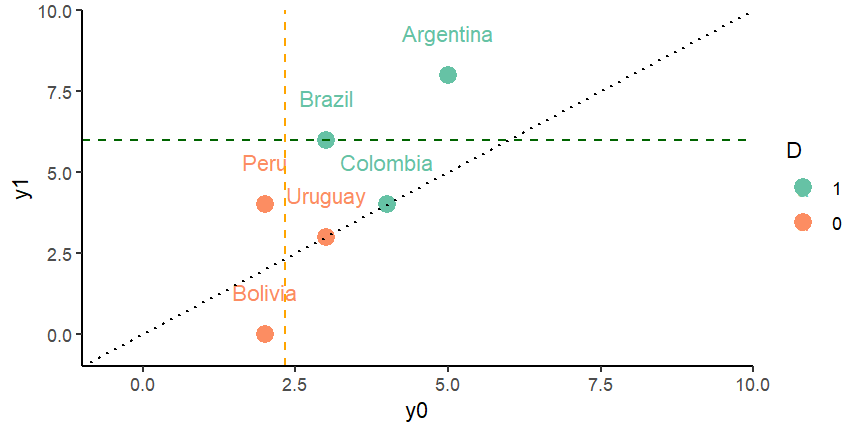
\includegraphics[width=\maxwidth]{figure/Chart_2-1} 
\end{knitrout}
\begin{itemize}
\item $E(Y_1|D=1)-E(Y_0|D=0) = 6 - 2.3 = 3.7$
\end{itemize}
\end{frame}

\begin{frame}
\frametitle{Causal Inference}
\footnotesize
\footnotesize
\begin{table}[htbp]
  \centering
    \begin{tabular}{|p{1.8cm}|p{1.8cm}|p{1.8cm}|p{1.8cm}|p{1.8cm}|}
    \hline
           & \multicolumn{1}{p{1.8cm}|}{Democracy?} & \multicolumn{1}{p{1.8cm}|}{GDP Growth if Dem} & \multicolumn{1}{p{1.8cm}|}{GDP Growth if NOT Dem} & \textbf{Treatment Effect} \bigstrut\\
    \hline
          \multicolumn{1}{|p{1.8cm}|}{} & \multicolumn{1}{p{1.8cm}|}{$D_i$} & \multicolumn{1}{p{2cm}|}{$Y_1$} & \multicolumn{1}{p{2.2cm}|}{$Y_0$} & \multicolumn{1}{p{1.8cm}|}{$Y_{1} - Y_{0}$} \bigstrut\\
    \hline
    Brasil & 1 & 6     & ?     & ? \bigstrut\\
    \hline
    Argentina & 1 & 8    & ?     & ? \bigstrut\\
    \hline
    Uruguay & 0 & ? & 3 & ?  \bigstrut\\
    \hline
    Bolivia & 0 & ?     & 2     & ? \bigstrut\\
    \hline
    Colombia & 1 & 4    & ?    & ? \bigstrut\\
    \hline
    Peru & 0 & ?     & 2     & ? \bigstrut\\
    \hline
    \textbf{Average Treatment Effect} & & \textbf{6} & \textbf{2.3} & \textbf{3.7} \bigstrut\\
    \hline
    \end{tabular}%
  \label{tab:addlabel}%
\end{table}%
\normalsize
\end{frame}

\begin{frame}
\frametitle{Selection Bias}
\begin{multicols}{2}
A real causal relationship:
\begin{knitrout}
\definecolor{shadecolor}{rgb}{0.969, 0.969, 0.969}\color{fgcolor}
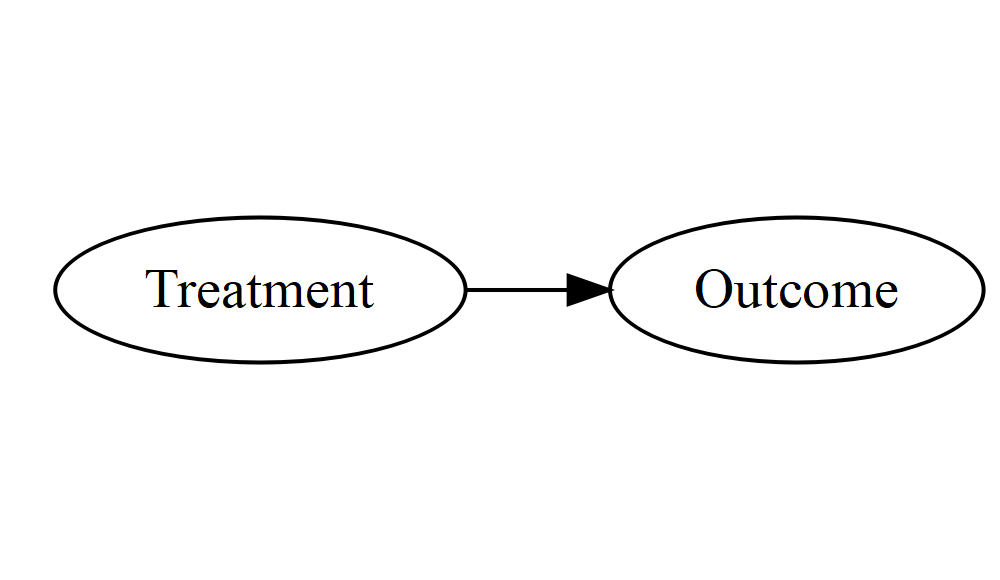
\includegraphics[width=\maxwidth]{figure/explanation7-1} 
\end{knitrout}
\columnbreak
Being misled by Selection Bias:
\begin{knitrout}
\definecolor{shadecolor}{rgb}{0.969, 0.969, 0.969}\color{fgcolor}
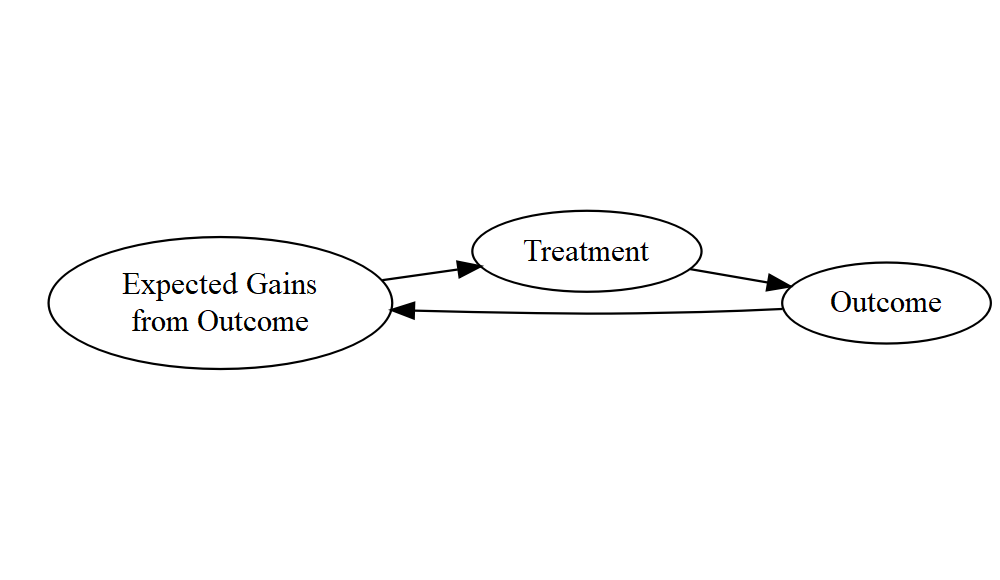
\includegraphics[width=\maxwidth]{figure/explanation8-1} 
\end{knitrout}
\end{multicols}
\end{frame}

\begin{frame}
\frametitle{Selection Bias}
\begin{multicols}{2}
A real causal relationship:
\begin{knitrout}
\definecolor{shadecolor}{rgb}{0.969, 0.969, 0.969}\color{fgcolor}
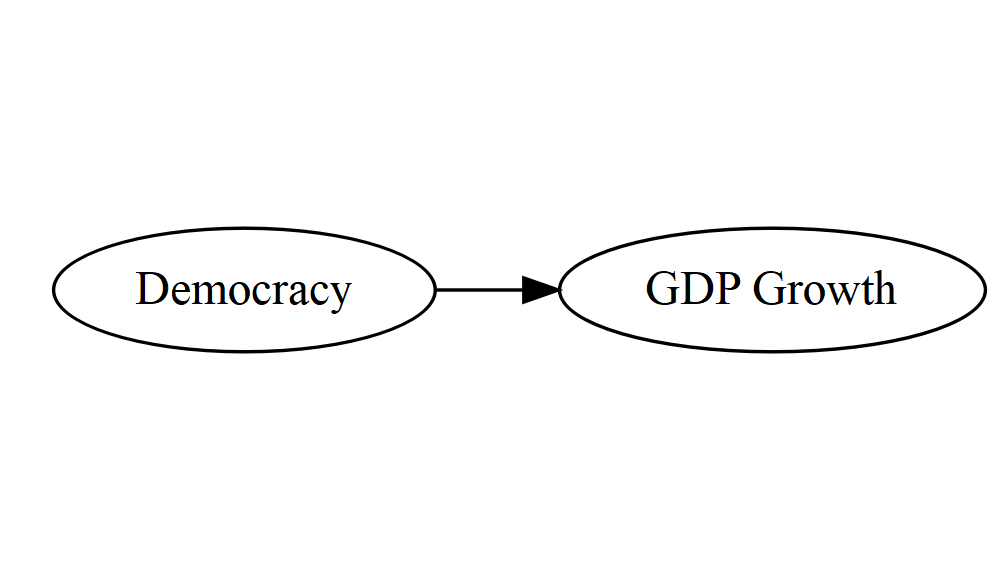
\includegraphics[width=\maxwidth]{figure/explanation9b-1} 
\end{knitrout}
\columnbreak
Being misled by Selection Bias:
\begin{knitrout}
\definecolor{shadecolor}{rgb}{0.969, 0.969, 0.969}\color{fgcolor}
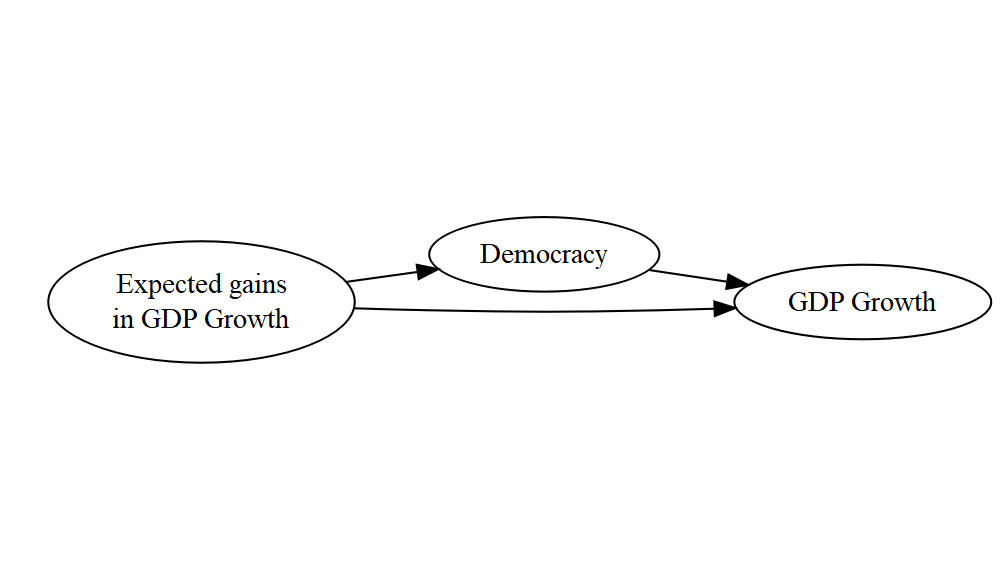
\includegraphics[width=\maxwidth]{figure/explanation10b-1} 
\end{knitrout}
\end{multicols}
\begin{itemize}
\pause
\item The units which benefit most from treatment (largest $y_1-y_0$) \textbf{choose treatment}
\pause
\item We don't see any of the low $y_1$'s of units which avoid treatment
\begin{itemize}
\pause
\item Countries which can boost their GDP growth by becoming a democracy choose to democratize
\pause
\item Ex. Mexico? Myanmar?
\end{itemize}
\end{itemize}
\end{frame}

\begin{frame}
\frametitle{Self-Selection Bias}
\footnotesize
\footnotesize
\begin{table}[htbp]
  \centering
    \begin{tabular}{|p{1.8cm}|p{1.8cm}|p{1.8cm}|p{1.8cm}|p{1.8cm}|}
    \hline
          & \multicolumn{1}{p{1.8cm}|}{Democracy?} & \multicolumn{1}{p{1.8cm}|}{GDP Growth if Dem} & \multicolumn{1}{p{1.8cm}|}{GDP Growth if NOT Dem} & \textbf{Treatment Effect} \bigstrut\\
    \hline
          \multicolumn{1}{|p{1.8cm}|}{} & \multicolumn{1}{p{1.8cm}|}{$D_i$} & \multicolumn{1}{p{2cm}|}{$Y_1$} & \multicolumn{1}{p{2.2cm}|}{$Y_0$} & \multicolumn{1}{p{1.8cm}|}{$Y_{1} - Y_{0}$} \bigstrut\\
    \hline
    Brasil & 1 & 6     & ?     & ? \bigstrut\\
    \hline
    Argentina & 1 & 8    & ?     & ? \bigstrut\\
    \hline
    Uruguay & 0 & ? & 3 & ?  \bigstrut\\
    \hline
    Bolivia & 0 & ?     & 2     & ? \bigstrut\\
    \hline
    Colombia & 0 & ?    & 4    & ? \bigstrut\\
    \hline
    Peru & 1 & 4     & ?     & ? \bigstrut\\
    \hline
    \textbf{Average Treatment Effect} & & \textbf{6} & \textbf{3} & \textbf{3} \bigstrut\\
    \hline
    \end{tabular}%
  \label{tab:addlabel}%
\end{table}%
\normalsize
\end{frame}

\begin{frame}
\frametitle{Self-Selection Bias}
\begin{knitrout}
\definecolor{shadecolor}{rgb}{0.969, 0.969, 0.969}\color{fgcolor}
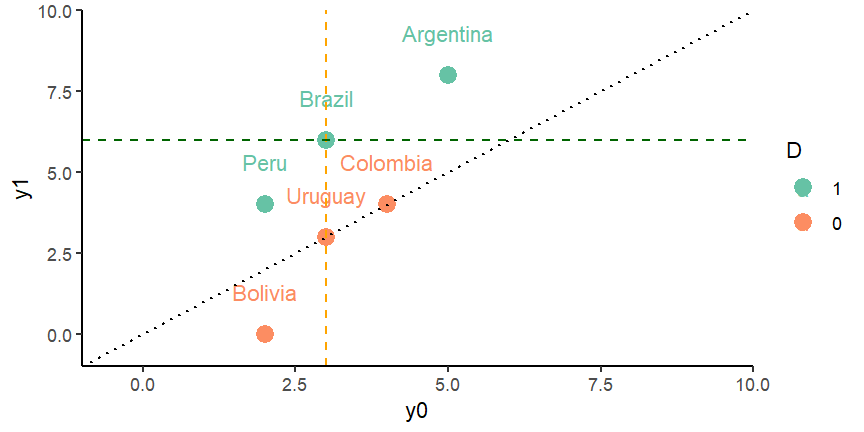
\includegraphics[width=\maxwidth]{figure/Chart_3-1} 
\end{knitrout}
\begin{itemize}
\item $E(y_1|D=1)-E(y_0|D=0)= 6 - 3 = 3$
\end{itemize}
\end{frame}

\begin{frame}
\frametitle{Self-Selection Bias}
\begin{itemize}
\item Allow treatment effects to vary across individuals, so $Y_{1i} = Y_{0i} + \alpha_i$
\end{itemize}
\pause
\begin{multline}
\underbrace{E(Y_i|D=1)-E(Y_i|D=0)}_\text{Observed Effect} \pause = \underbrace{E(Y_{1i} - Y_{0i})}_\text{Real ATE} \\ + \underbrace{\frac{1}{2}\Big[ E(Y_{1i}|D=1) - E(Y_{1i}|D=0) \Big]}_\text{Imbalance on $Y_1$} + \underbrace{\frac{1}{2}\Big[ E(Y_{0i}|D=1) - E(Y_{0i}|D=0) \Big]}_\text{Imbalance on $Y_0$}
\end{multline}
\footnotesize
NB: For equal-sized treatment and control groups
\normalsize
\end{frame}

\begin{frame}
\frametitle{Self-Selecion Bias}
\begin{itemize}
\item Selection Bias occurs where our data sample does not tell the complete story:
\pause
\begin{enumerate}
\item \textbf{Self-selection Bias:} Units that benefit most from treatment choose to receive treatment
\begin{itemize}
\item Those with the biggest difference  in potential values, $Y_1 - Y_0$
\end{itemize}
\item \textbf{Data Availability Bias:} Some types of units don't report data
\begin{itemize}
\item \textit{For reasons related to the treatment and potential outcomes}
\pause
\item Eg. Wealthy autocracies and poor democracies do not like to report data
\pause
\item Only wealthy democracies 'select' into our sample
\end{itemize}
\item \textbf{Survival Bias:} Some types of units drop out of our sample
\begin{itemize}
\item \textit{For reasons related to the treatment and potential outcomes}
\end{itemize}
\end{enumerate}
\end{itemize}
\end{frame}

\setbeamercolor{background canvas}{bg=}
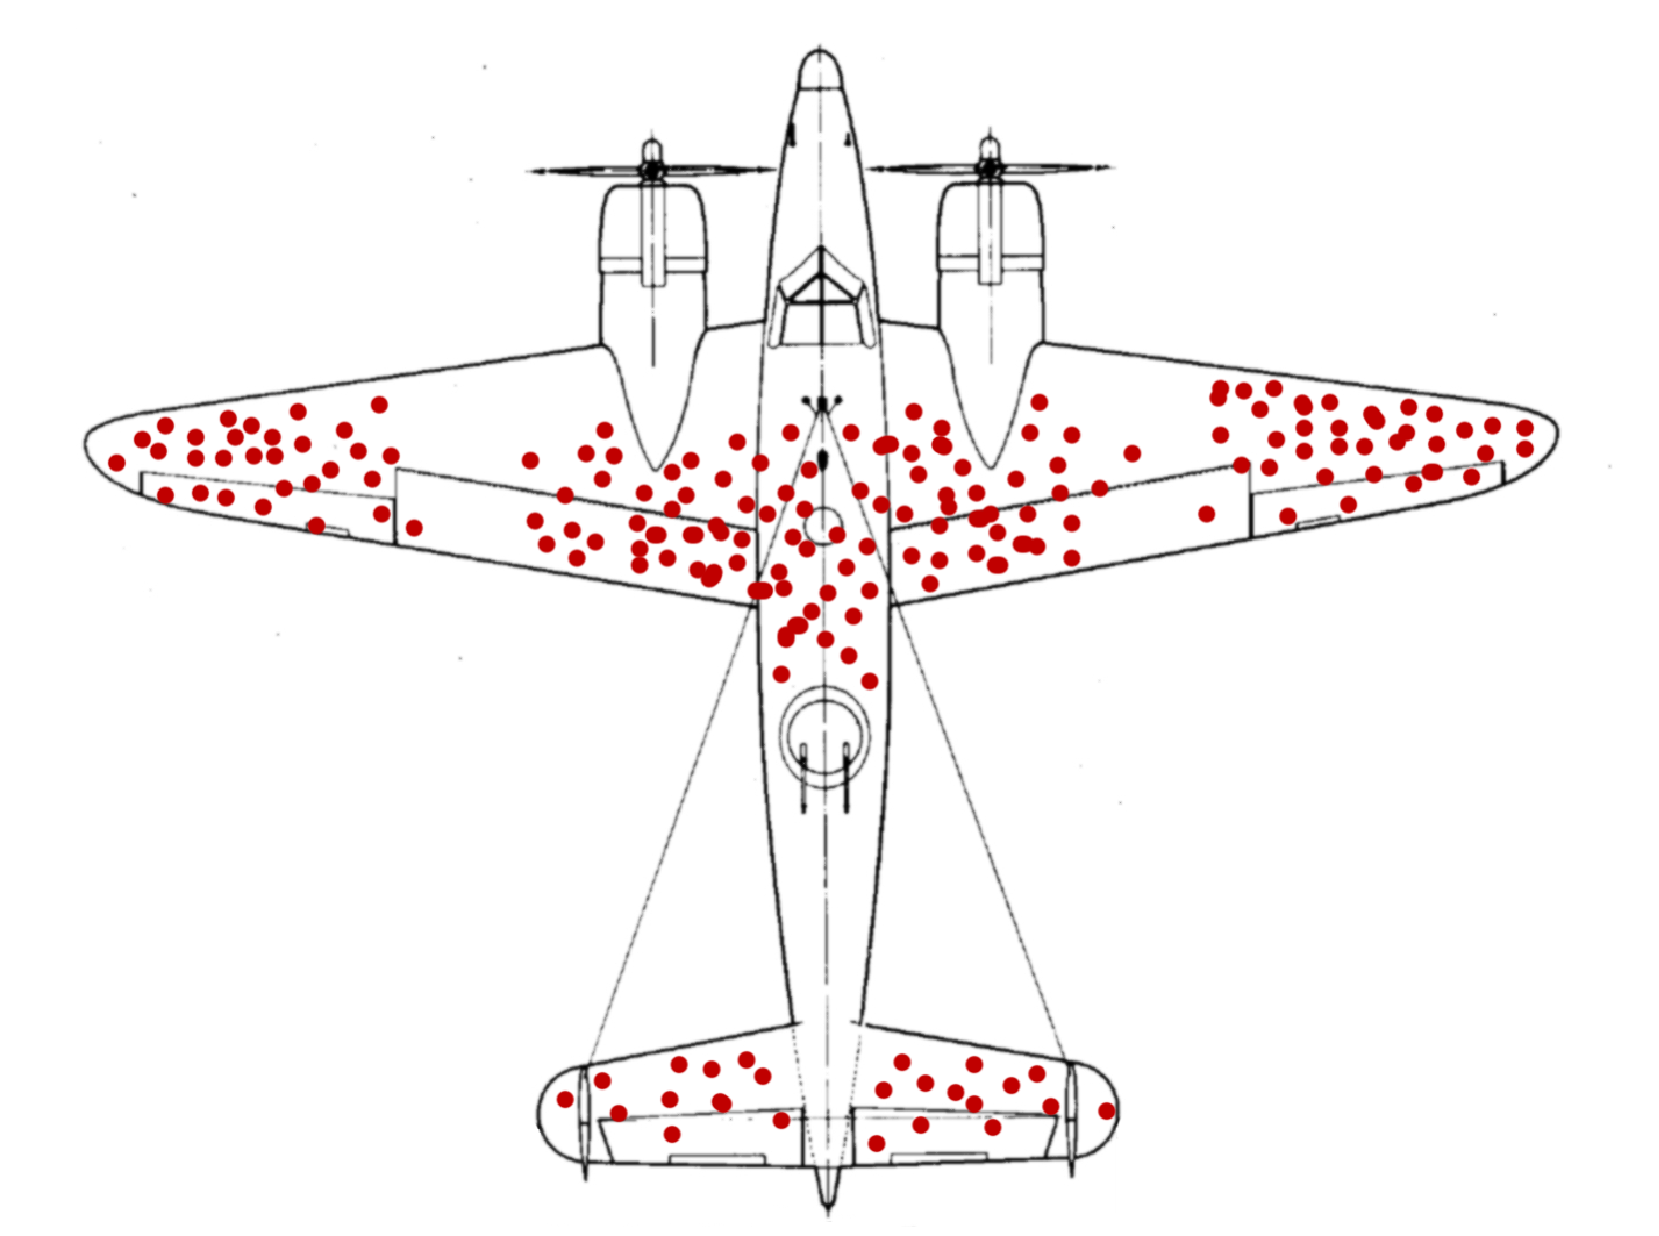
\includepdf[pages={1}]{Bombers.pdf}



\begin{frame}
\frametitle{Problems with Observational Data}
\begin{itemize}
\item Depending on the treatment assignment mechanism we get a range of Average Treatment Effects:
\end{itemize}
\begin{table}[htbp]
  \centering
  \caption{Comparing Average Treatment Effects}
    \begin{tabular}{|l|r|}
    \hline
    \textbf{Treated Units} & \multicolumn{1}{l|}{\textbf{ATE}} \bigstrut\\
    \hline
    Real Effect for all units & 1 \bigstrut\\
    \hline
    Bolivia and Colombia treated & -1.25 \bigstrut\\
    \hline
    Omitted Variable Bias (Southern Cone) & 3 \bigstrut\\
    \hline
    Reverse Causation & 3.7 \bigstrut\\
    \hline
    Self-selection (Biggest GDP gains) & 3 \bigstrut\\
    \hline
    \end{tabular}%
\end{table}%
\end{frame}

\begin{frame}
\frametitle{3 Critiques}
\begin{itemize}
\item \textit{ANY} time you see a paper based on observational data, you should try to make the three critiques:
\pause
\begin{enumerate}
\item Omitted Variables
\item Reverse Causation
\item Selection Bias
\end{enumerate}
\item In all these cases, treatment assignment is not independent of potential outcomes
\end{itemize}
\end{frame}


\end{document}
 
